\documentclass[11pt,a4paper,titlepage,oneside]{report}
\usepackage{titling}
\usepackage{graphicx}
\usepackage{mathtools}
\usepackage{lmodern}
\usepackage{amsmath}
\usepackage{float}
\usepackage{subfig}
\usepackage{listings}
\usepackage[hidelinks]{hyperref}

%% Memoir layout setup

%% NOTE: You are strongly advised not to change any of them unless you
%% know what you are doing.  These settings strongly interact in the
%% final look of the document.

% Dependencies
\usepackage{bfhlogo}
\usepackage{etoolbox}% http://ctan.org/pkg/etoolbox

\makeatletter
%%begin novalidate
%% Titlepage adjustments
\pretitle{\vspace{0pt plus 0.7fill}\begin{center}\Huge}
\posttitle{\end{center}\par}
\preauthor{\par\begin{center}\let\and\\\Large}
\postauthor{\end{center}}
\predate{\par\begin{center}\Large}
\postdate{\end{center}}
%%end novalidate
\def\@advisors{}
\newcommand{\advisors}[1]{\def\@advisors{#1}}
\def\@department{}
\newcommand{\department}[1]{\def\@department{#1}}
\def\@thesistype{}
\newcommand{\thesistype}[1]{\def\@thesistype{#1}}

\renewcommand{\maketitlehooka}{\noindent\bfhlogo[2cm]}

\renewcommand{\maketitlehookb}{\vspace{1in}%
  \par\begin{center}\Large\sffamily\@thesistype\end{center}}

\renewcommand{\maketitlehookd}{%
  \vfill\par
  \begin{flushright}
    \sffamily
    \@advisors\par
    \@department, BFH
  \end{flushright}
}

% Fix the chapters (unnecessary space)
\patchcmd{\@makechapterhead}{\vspace*{50\p@}}{}{}{}% Removes space above \chapter head
\patchcmd{\@makeschapterhead}{\vspace*{50\p@}}{}{}{}% Removes space above \chapter* head

\makeatother

\setlength{\droptitle}{-48pt}


\setlength{\parindent}{0pt}

\title{ORB Slam Point Cloud generation on Apalis iMX8}
\author{Stefan Eichenberger}
\date{Januar 2019}
\advisors{Marcus Hudritsch}
\department{TSM CPVR Lab}

\lstset{
	basicstyle=\ttfamily\scriptsize
}

\begin{document}
\maketitle

\begin{abstract}
	For navigating a robot around obstacles we require a map of its environment. Because robots can be small and independent of power plugs, they have limited processing power. This work analyzes how suitable ORB SLAM is for an embedded processor and what improvements are required to make it work on such a platform.
\end{abstract}

\section*{Executive Summary}
Simultaneous Location and Mapping (SLAM) is an important topic in computer vision today. The possibilities for this technology are infinite. We can use SLAM for navigation, object recognition and augmented reality. Often this algorithms need a high performance graphics card or a high performance processor. For industrial and robotics purposes we have constraints in space, temperature and power consumption. This doesn’t allow the use of high performance CPUs. This work analyzes the ORB SLAM algorithm on how it performs on a modern embedded ARM CPU. The long-term goal is to have a system available that generates a map and to use this map for further navigation.

\tableofcontents

\chapter{Introduction}
To find the position of a robot we can use different sensors. Navigation systems use IMUs, magneto meters, radio signals and for outdoor navigation GPS. Humans however, do a lot of navigation by eye. Embedded systems today have enough processing power to make complex calculations. Therefore, a possibility to estimate the position of the robot can also be computer vision. One field in computer vision is SLAM where we try to create a map of the environment and to estimate the pose of the camera based on camera images. In this project, we analyze the performance of ORB SLAM \cite{orbslam} running on an iMX8 QuadMax as embedded system. We use a stereo camera to create a point cloud and use this point cloud to calculate the changes in pose and position. As we will see, by using a stereo camera we can reconstruct a point cloud with a known scale. This allows us to create a 3D map with real world scale of the environment around the camera.

\section{Apalis iMX8 QuadMax}
Toradex supports this project with embedded hardware. Toradex is a system on module provider focusing on embedded ARM devices for industrial applications. They are interested to see some applications and demos running on the Apalis iMX8 QuadMax (figure \ref{fig:apalis_imx8}). Therefore, we try to port the SLAM application onto this platform. One area where NXP, the manufacturer of the processor, tries to focus the iMX8 is computer vision in industry and automation. Therefore, this CPU should be a good fit for this kind of application. NXP launches different iMX8 variants. Publicly available today is only the iMX8M which is performance wise placed between the iMX8 and the iMX8X. The Apalis iMX8 QuadMax used in this project is the processor with highest performance. They will release it in 2019. This work uses an alpha silicon of the processor which is provided by Toradex.

\begin{figure}[H]
  \begin{center}
		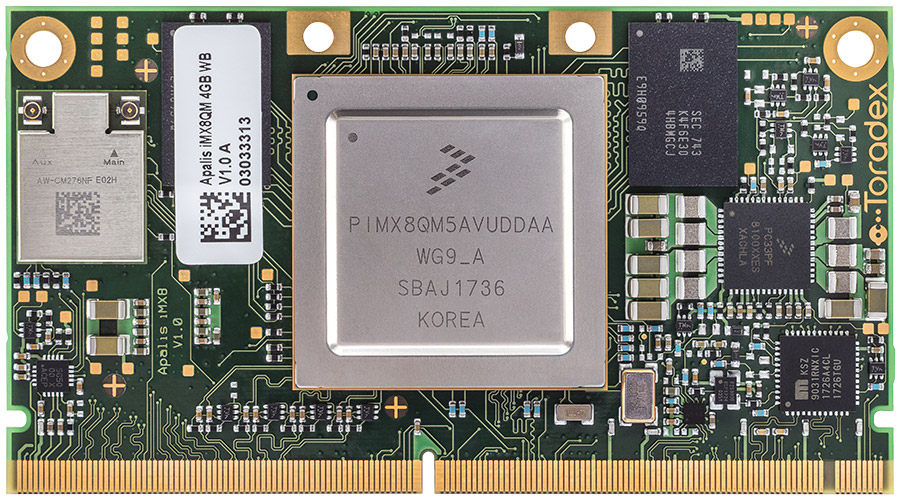
\includegraphics[width=1.0\textwidth]{img/apalis_imx8.jpg}
  \end{center}
	\caption{Apalis iMX8 from Toradex}\label{fig:apalis_imx8}
\end{figure}


\subsection{Features}

The iMX8 QuadMax has the following specification:
\begin{itemize}
  \item Two Cortex A72 high performance processors
  \item Four Cortex A53 low power processors
  \item Two Cotex M4 realtime MCUs
  \item Two Vivante GC7000 GPUs each with 8 cores with each capable to process vectors of length 4
  \item Industrial temperature range from -40°C to 85°C
	\item 16GB eMMC Flash
	\item 4GB LPDDR4 RAM
\end{itemize}

The iMX8 is focusing on industrial applications. Therefore, it doesn’t use state-of-the-art production processes. They produce the iMX8 in 28nm structure while Smartphone processors today use 7nm technology. However, bigger structures make the processor less prone to high temperatures. The two Cortex A72, the four Cortex A53 and the Vivante GPU have the performance level of a today's mid-end Smartphone. The two Cortex M4 processors could be used to do Realtime processing. However, we don’t use them in this work.

\section{Goals}
We can describe the goal of this project as follows:
\begin{itemize}
\item Porting ORB SLAM to the Apalis iMX8 QuadMax
\item Analyzing different possibilities to speed up the ORB SLAM algorithm
\item Add an extension that creates a dense point cloud which could later be used to extract detailed maps
\item Allow SLAM in realtime with min. 20fps to track fast movements
\item Evaluate the results and start discussion about further work
\end{itemize}

The focus of this work is to figure out how we can use or implement a SLAM algorithm that later could reconstruct the world around the camera in 3D. This 3D world or 3D point cloud could in a later step, that is not part of this work, used to plan paths around obstacles and to estimate the position of a camera in a known environment.

\section{Time Plan}

The project was planned to end in early January. The concept phase started well. Unfortunately, standard ORB SLAM didn’t perform well for our purposes. First optimizations only improved the performance a little. However, we implemented a dense point cloud generator based on this implementation to figure out what challenges we have to fight there. The time plan of this project is shown in figure \ref{fig:timeplan}.
\begin{figure}[H]
	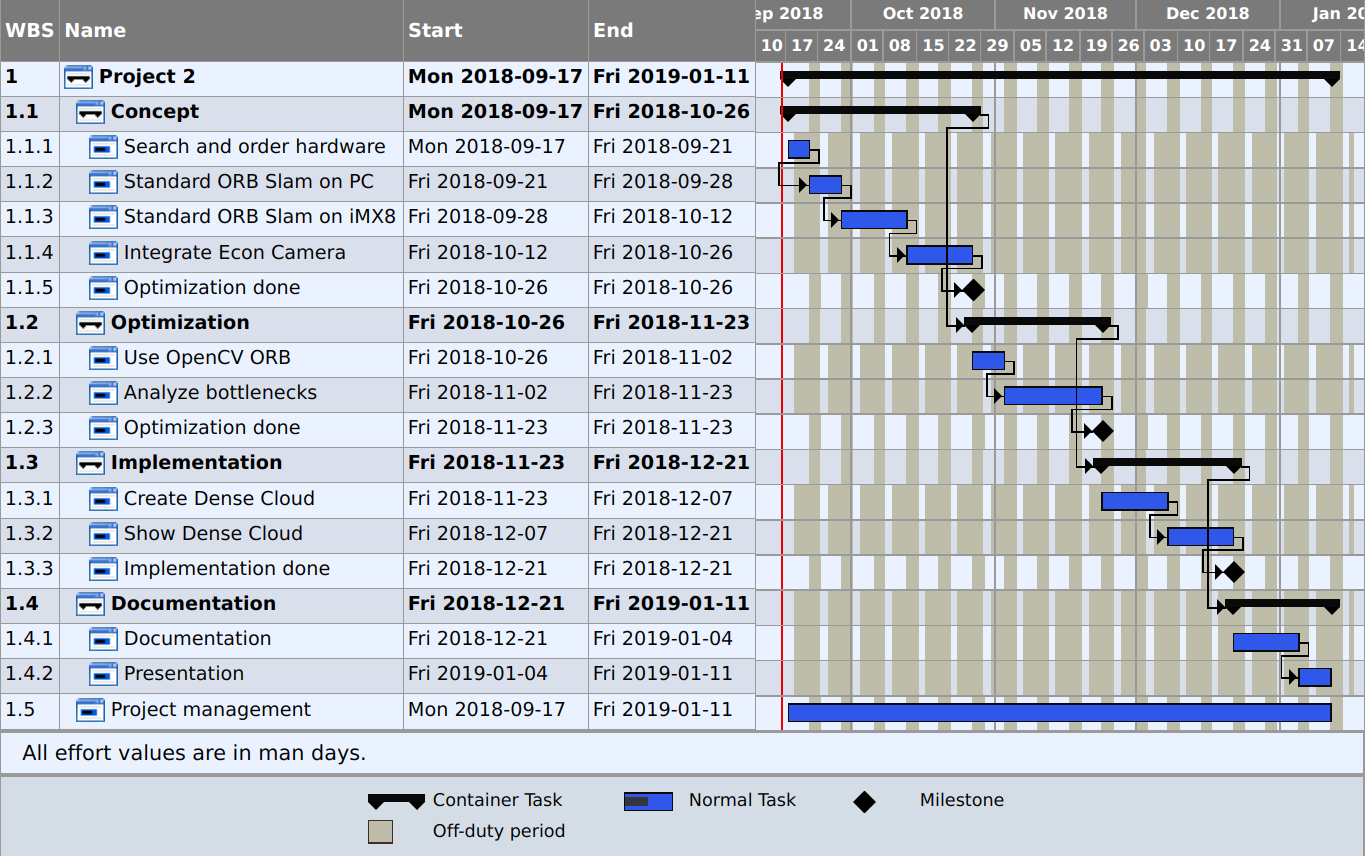
\includegraphics[width=1.0\textwidth]{img/timeplan.png}
	\caption{Time Plan}\label{fig:timeplan}
\end{figure}

\chapter{SLAM Evaluation}

In this section we analyze different documented SLAMs. We can split them in two groups, indirect and direct SLAM (figure \ref{fig:slammodes}). Indirect methods analyze an image and try to extract features. This feature points are matched directly to further images. Based on these matches we can estimate the pose of the camera. Direct methods operate on intensity variances. The goal is to find a pose that minimizes the intensity difference between two images. Because minimizing the intensity difference over the whole image is computational expensive most methods operated only on edges or corners of the image. We call such methods direct semi dense or direct sparse. In the next sections we will have a discussion about these different approaches.

\begin{figure}[H]
	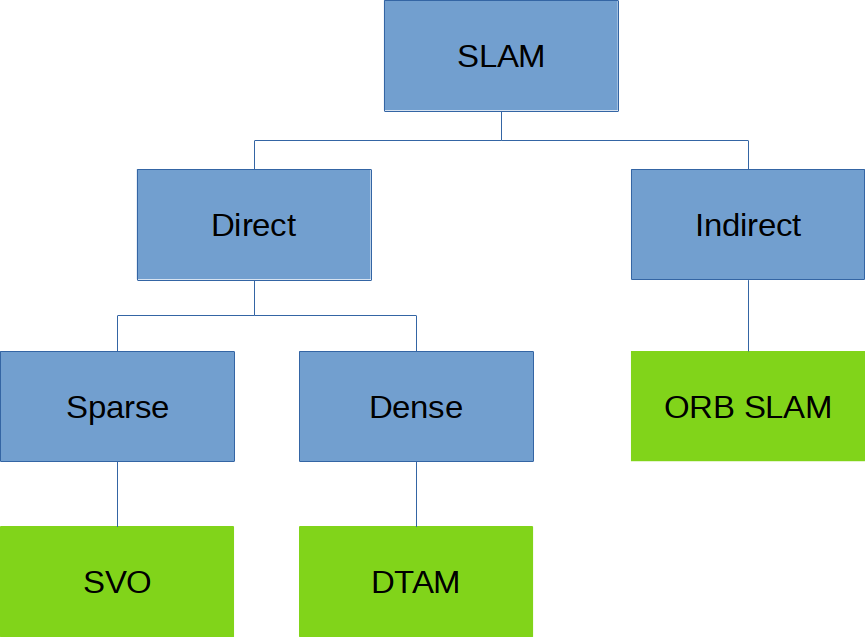
\includegraphics[width=1.0\textwidth]{img/slam_modes.png}
	\caption{SLAM Modes}\label{fig:slammodes}
\end{figure}


\section{Indirect method}

A well documented indirect method is ORB SLAM \cite{orbslam}. ORB SLAM extracts ORB keypoints which are then matched with a known 3D point cloud. Based on these matches it can do triangulation with RANSAC \cite{ransac} to estimate the current pose and position. Indirect methods can estimate the pose through triangulation which isn’t computationally expensive. On the other side computing descriptors costs CPU time. We will describe ORB SLAM in more detail in chapter \ref{chap:implementation}.

\section{Direct method}

In this section we will analyze two direct approaches a dense and a sparse approach. Dense methods use all pixels on the image for tracking while sparse methods only use a subset. Figure \ref{fig:sparse_dense} shows a comparison of dense sparse and semi-dense approaches. We don't dig into semi-dense approaches they work similar to sparse methods but with more keypoints.

\begin{figure}[H]
  \begin{center}
		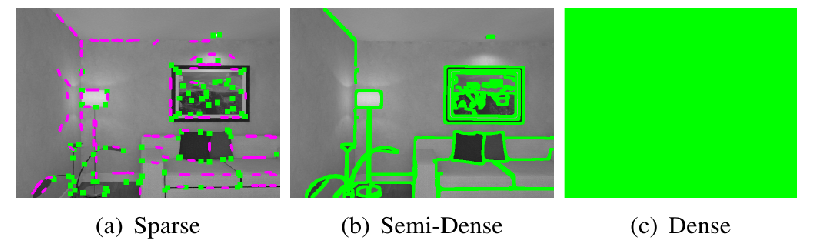
\includegraphics[width=1.0\textwidth]{img/sparse_dense.png}
  \end{center}
	\caption{Comparison of sparse, dense and semi-dense approaches \cite{svo}}\label{fig:sparse_dense}
\end{figure}

\subsection{Dense}

There are not that many dense SLAMs. One is DTAM \cite{dtam} which uses the intensity values of the whole image to estimating the pose. The idea is to minimize the intensity difference (energy) between two images by optimizing the camera pose. The energy defined at one pixel position is defined as shown in equation \ref{eq:pixel_energy}. To estimate the pose and position it tries to find a projection matrix that minimizes $E_{t}$ as shown in equation \ref{eq:total_energy}.
\begin{equation}\label{eq:pixel_energy}
\begin{aligned}
  E_{xy}=I_1(x,y)-I_2(x',y')\\
	\begin{pmatrix}
	x'*s'\\
	y'*s'\\
	s'\\
	\end{pmatrix}=P*XYZ
\end{aligned}
\end{equation}
Where:
\begin{align*}
  E_{xy}	&: \text{Energy at a specific position}\\
  I_1			&: \text{Previous image}\\
  I_2			&: \text{Current image}\\
  x,y			&: \text{Point position in previous image} \\
  x',y'		&: \text{Point position in current image} \\
	s'			&: \text{Scaling value}\\
  P				&: \text{Projection matrix}\\
  XYZ			&: \text{Point position in 3D cloud}
\end{align*}
\begin{equation}\label{eq:total_energy}
  E_{t}=\min(\sum_{x=0}^C\sum_{y=0}^RE_{xy})
\end{equation}
Where:
\begin{align*}
  E_{t}		&: \text{Total energy}\\
  E_{xy}	&: \text{Energy at pixel position x/y in image}\\
	C				&: \text{Image columns}\\
	R				&: \text{Image rows}\\
\end{align*}

Direct dense method deliver a dense point cloud which we can use directly to create maps and 3D objects. However, they are computational expensive. Therefore, they are not appropriate for embedded devices.

\subsection{Sparse}

Sparse direct SLAMs like SVO \cite{svo} don’t optimize the Energy over the whole image but the energy at sparse points instead. One possibility of a sparse point is e.g. a corner point found by FAST \cite{fast}. Similar to sparse methods there are semi dense methods which try to minimize the energy on several points laying on edges. Canny Edge detection or DoG can for example find such edges. The advantage of sparse and semi dense methods is that they are less computationally expensive than dense methods.\\\\
Sparse direct methods don’t create dense clouds immediately however they can work on weaker keypoints than indirect methods. Therefore, they can create denser clouds than e.g. ORB SLAM. They can also be computational less expensive than indirect methods because they don’t have to calculate expensive features \cite{svo}.

\section{Stereo and Monocular SLAM}

In this project, the focus is on stereo SLAM. A lot of today's paper focus on monocular SLAM. The reasons are that monocular cameras are cheaper and monocular cameras are available in Smartphones. Monocular SLAM has two problems we don’t have with stereo SLAM. First an initialization process has to estimate the movement between two frames. We can only create a 3D point cloud based on two images with known position, in the monocular case the position of two images is random. Therefore, the algorithm needs to guess the pose and transformation over a few images until it knows the poses. It does that by making assumptions on the world or by trying to optimizing the point positions over several images. However, even when successfully initialized the second problem persists. Monocular SLAM is not able to guess the scale of the point cloud. The intuition for this issue is that we can’t distinguish between the movement of the camera on a small model close to the scene or the movement of the camera on the original model further away from the scene. With stereo SLAM we don’t have this issue. For each camera pose we get two images with a known distance between the two camera sensors (baseline). Therefore, we can calculate the depth of each pixel in real world distance. From this we can generate a point cloud assuming that the initial camera pose is at origin. We therefore have an instantaneous initialization and can calculate the real world position in a known unit e.g. meters. Tracking between two camera poses is however the same on monocular and stereo SLAM. However we can again insert new keypoints immediately on stereo cameras without the need of using a second camera pose.

\section{Decision}

In this project, we port ORB SLAM onto iMX8 and see how it performs. We use ORB SLAM because of the following reasons:
\begin{itemize}
	\item Open source implementation available
	\item Powerful framework for displaying point cloud and images
	\item Good documentation
	\item Indirect methods seem promising because triangulation is fast
	\item The CPVR lab already has experience with ORB on Smartphones
\end{itemize}

Based on ORB SLAM we try to analyze how we can use the iMX8 and whether ORB SLAM fits well for this platform.

\chapter{Camera Evaluation}

To do stereo computer vision, we need a stereo camera. There are a few stereo cameras available on the market. It is also possible to build a stereo camera with two monocular cameras. However, we decided against that because it would require a mechanism to synchronize the images from both streams. We analyze three stereo cameras available on the market.

\section{ZED}
The ZED camera \cite{zed} is a stereo camera from Stereo Labs. Here the specification of this camera:
\begin{itemize}
	\item Full HD color images with 30fps
	\item USB3.0
	\item UVC compliant
	\item Linux SDK
	\item Baseline 120mm
	\item IMU sensor with 6DoF
	\item Price: 449\$
\end{itemize}

To run their SDK a Dual Core CPU with 2.3 GHz and CUDA > 3.0 is required. However, it's also possible to use the camera without their SDK.

\section{ECON Tara}
The Tara camera \cite{tara} from Econ is another stereo camera. In comparison to the ZED camera it delivers a reduced resolution and only gray scale images.
\begin{itemize}
	\item 752x480 gray scale images with 60fps
	\item USB3.0
	\item Global Shutter Camera
	\item UVC compliant
	\item Baseline 60mm
	\item IMU sensor with 6DoF
	\item Open Source SDK
	\item Price: 149\$
\end{itemize}

It has a small OpenCV based SDK with open source software. In comparison to the ZED SDK it is less powerful.

\section{Intel RealSense D435}
The Intel RealSense camera \cite{realsense} is a infrared stereo camera. In comparison to RGB stereo cameras it uses infrared images for stereo vision. It seems that this sensors are less prone to reflections. A third camera delivers RGB images in full HD.
\begin{itemize}
	\item 1280x720 with 90fps (IR), 1920x1080 with 30fps (RGB)
	\item USB3.0
	\item Global Shutter Camera
	\item UVC compilant (kernel patch required)
	\item Baseline 50mm
	\item Open Source SDK (librealsense)
	\item Price: 179\$
\end{itemize}

The Intel SDK seems quite powerful and is open source as well. However, the indepth details of the camera are not publicly available.

\section{Decision}

We decided to use the Econ Tara because it has an outstanding price ratio and because it is a conventional stereo camera. However, the Intel RealSense camera is also a great fit because it delivers depth images directly. This reduces the CPU load on the iMX8. If we require Full HD, we should use the ZED camera. Another advantage of the ZED camera is the bigger baseline of 120mm. This allows depth estimation with higher range. We decided against this camera mainly because of the high price and because of the closed source SDK. We can't benefit from Full HD sensors because embedded systems only have limited CPU resources.

\chapter{Camera Calibration}

Camera calibration is necessary to find a model that expresses the properties of a camera. Properties of a camera are:

\begin{itemize}
	\item Focal length of the camera lense
	\item Principal point on the camera sensor, where the z axis of the cameras coordinate system goes through.
	\item Distortion of the camera lense
	\item Size of a pixel
\end{itemize}

One example where we need to know the camera model is if we project virtual objects into a real world image. Figure \ref{fig:model} shows an image of a checkerboard where we project a virtual cube onto. One camera model in this image took distortion into account while the other one ignored it.
\begin{figure}[H]
  \begin{center}
		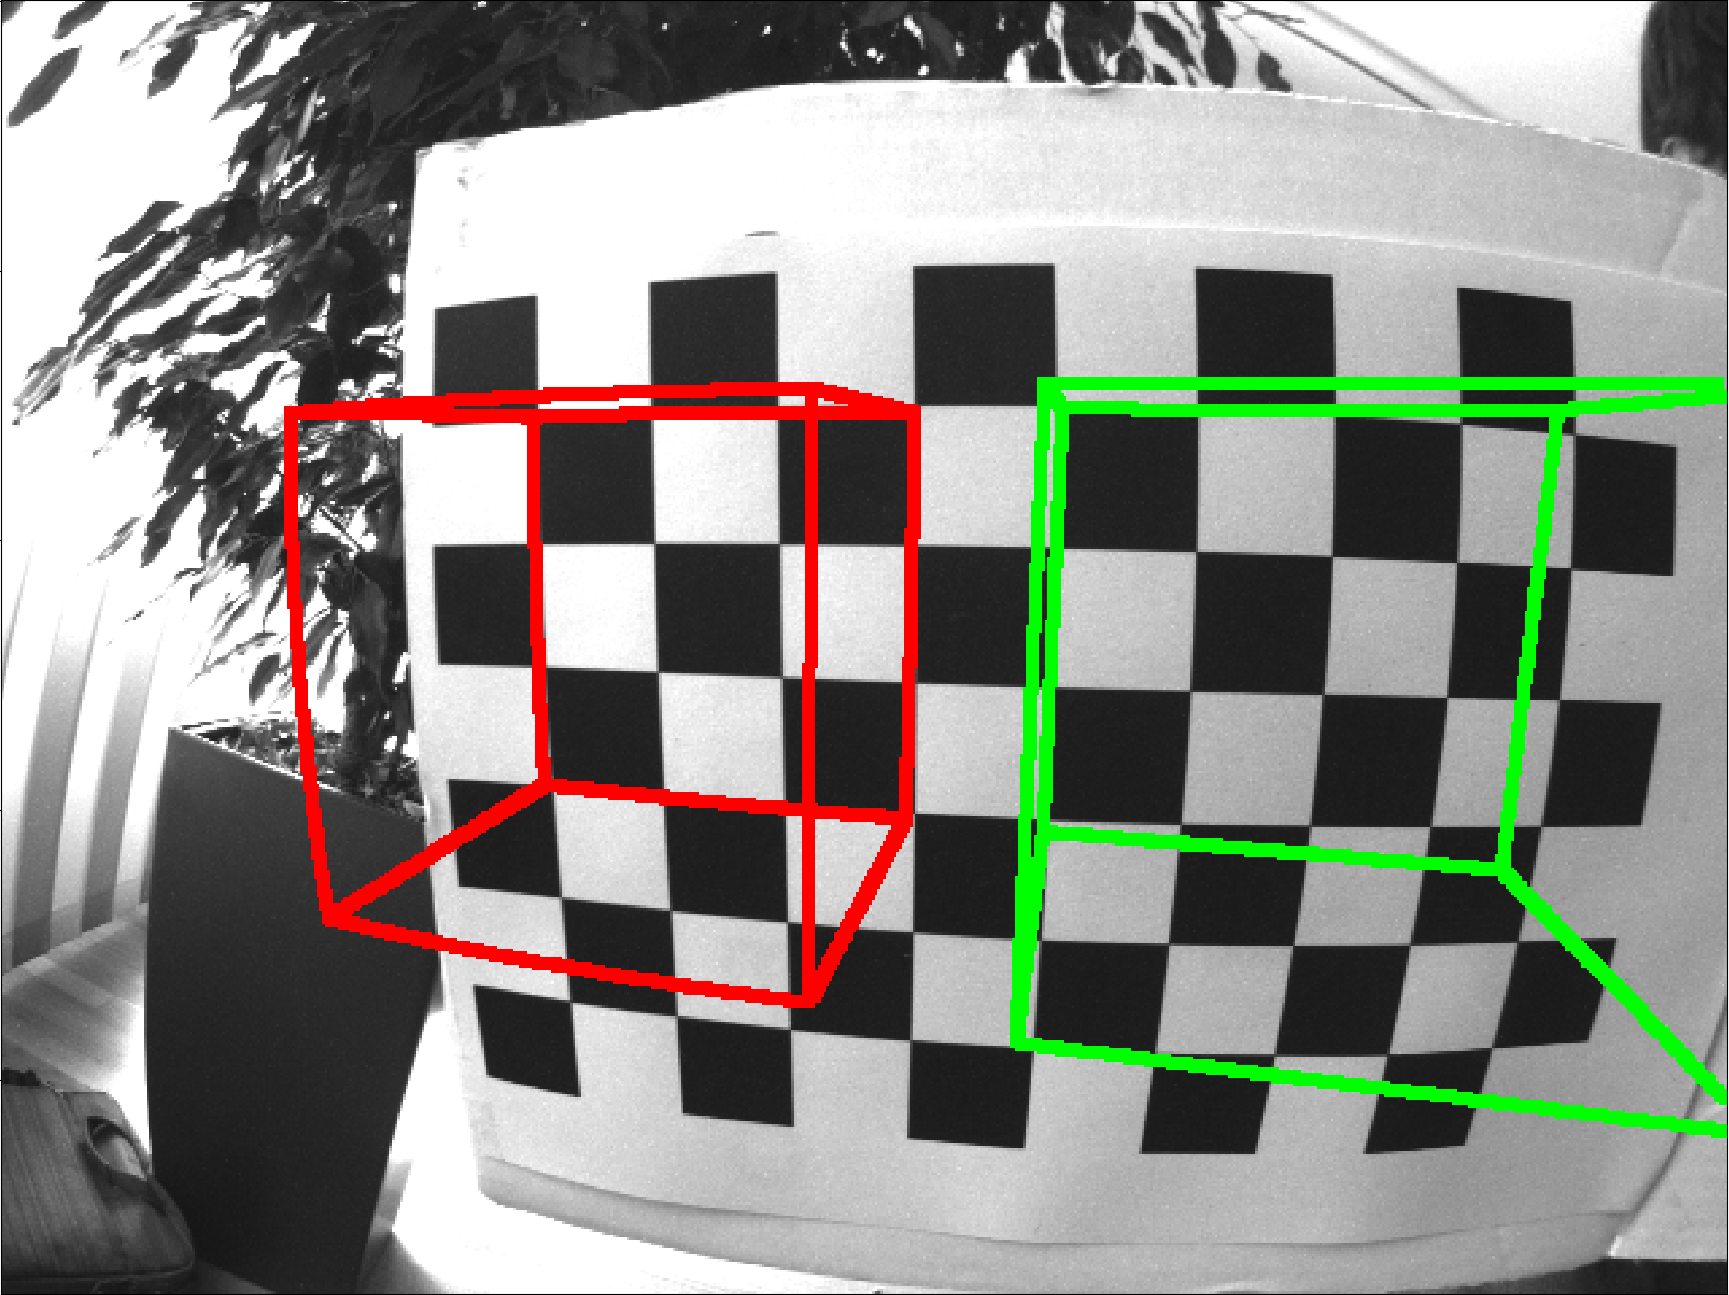
\includegraphics[width=1.0\textwidth]{img/model.png}
  \end{center}
	\caption{Applied camera model with (red) and without(green) distortion}\label{fig:model}
\end{figure}

We also need to know the camera model when doing SLAM. With known camera model we can rectify (see \ref{fig:calibration_real}) the image so we can assume the camera as a ``perfect’’ pinhole camera model with known image center and known focal width. Additional to the above parameters we need to align the images of the left and right camera in stereo vision. The cameras aren’t perfectly aligned in the vertical direction. However, we need to have them aligned because this makes it possible to search for matches only on the epipolar line \cite{mvg}. Further the cameras are slightly rotated which means we must inverse rotate the image to have a perfect alignment. So additional to the properties of a monocular camera we need to know the following parameters:
\begin{itemize}
	\item Y offset of the right camera to the left camera in pixels
	\item Rotation matrix of the right camera with left as reference
	\item The distance between left and right camera center (baseline)
\end{itemize}

\section{Camera Model}

The camera model expresses how any point in the three-dimensional space is projected onto a two-dimensional image. As a first approximation it assumes that all rays are going through one point. This is called the pinhole camera model (figure \ref{fig:projection}a). Given this assumption we can describe the projection of a 3D point onto a 2D image as shown in equation \ref{eq:cm}. We calculate the pixel location $x,y$ on the image by normalizing with $s$ as show in equation \ref{eq:cm_normalized} \cite{rvc}.
\begin{equation}\label{eq:cm}
  \begin{pmatrix}
		f_x & \gamma & c_x \\
		0 & f_y & c_y \\
		0 & 0 & 1 \\
	\end{pmatrix}*
	\begin{pmatrix}
		r_{00} & r_{01} & r_{02} & t_x \\
		r_{10} & r_{11} & r_{12} & t_y \\
		r_{20} & r_{21} & r_{22} & t_z \\
	\end{pmatrix}
	\begin{pmatrix}
		X \\
		Y \\
		Z \\
		1
	\end{pmatrix}=
	\begin{pmatrix}
		u \\
		v \\
		s
  \end{pmatrix}
\end{equation}
\begin{equation}\label{eq:cm_normalized}
	\begin{pmatrix}
		x \\
		y
	\end{pmatrix}=
	\begin{pmatrix}
		u/s \\
		v/s 
  \end{pmatrix}
\end{equation}

Where:
\begin{align*}
  X,Y,Z			&: \text{point in the 3D world}\\
	u,v,s	   	&: \text{point in 2D image not normalize}\\
	x,y				&: \text{point in 2D image normalized with s}\\
	f_x,f_y  	&: \text{focal length of the camera}\\
  c_x,c_y  	&: \text{principal point}\\
  t_x,t_y,t_z	&: \text{location of the camera}\\
  r_{ij}	&: \text{part of the rotation matrix}
\end{align*}

We can describe the intuition as follows. A Point (X,Y,Z) is projected onto an image sensor (u/s,v/s) by the multiplication of the intrinsic times the extrinsic matrix. The extrinsic matrix describes where the pinhole of the camera is located in the three dimensional space. The intrinsic camera matrix describes how the camera is constructed. For example, in figure \ref{fig:projection}b we translate and rotate a point $p_i$ with the extrinsic matrix so we can describe its coordinates with the pinhole as origin. Further we transform the point with the intrinsic camera matrix onto the image sensor.

\begin{figure}[H]
	\centering
	\subfloat[Pinhole model]{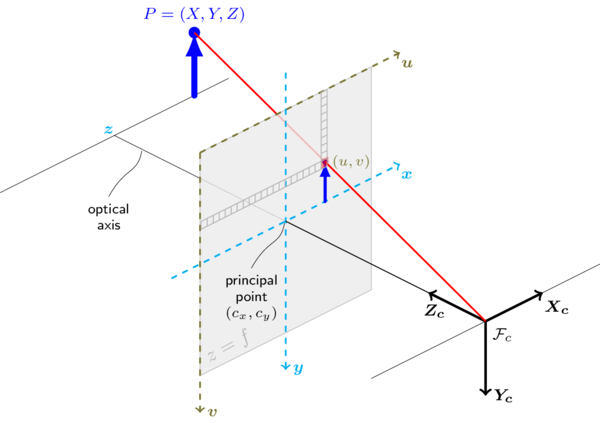
\includegraphics[width=0.5\textwidth]{img/pinhole_camera_model.png}}
	\subfloat[3D point to 2D point]{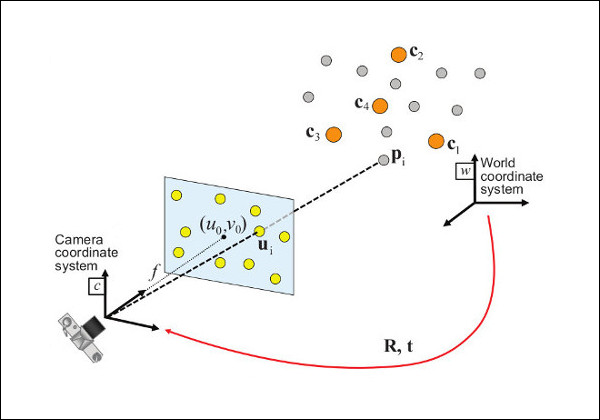
\includegraphics[width=0.5\textwidth]{img/pnp.jpg}}
	\caption{Image projection}\label{fig:projection}
\end{figure}

The goal of camera calibration is to find the intrinsic camera matrix. When doing SLAM we try to find the extrinsic matrix. When doing triangulation we normally get the projection matrix. With known intrinsic matrix we can calculate the position and pose (extrinsic matrix) of the camera by multiplying the projection matrix with the inverse of the intrinsic matrix as shown in equation \ref{eq:extrinsic}. 

\begin{equation}\label{eq:extrinsic}
	E=I^{-1}*P
\end{equation}

\begin{align*}
	E		&: \text{Extrinsic Matrix}\\
	I		&: \text{Intrinsic Matrix}\\
	P		&: \text{Projection Matrix}
\end{align*}

A good reference for camera calibration is the OpenCV documentation \cite{opencv_calib}. We won't describe this process in more detail.

\section{Stereo Camera Model}

Additional to the monocular parameters we need to find the parameter of the stereo camera. An image taken by a stereo camera normally is misaligned as shown in the top row of figure \ref{fig:stereo_calib}. The goal is to find the rotation matrix as well as the Y offset to get a perfectly aligned image pair as shown in the bottom row of figure \ref{fig:stereo_calib}.

\begin{figure}[H]
  \begin{center}
		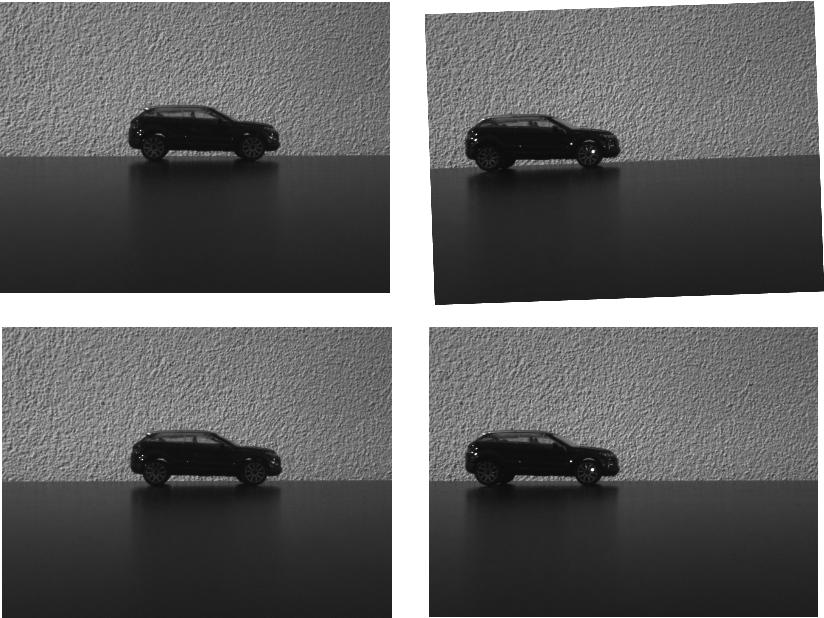
\includegraphics[width=0.9\textwidth]{img/car_calib.jpg}
  \end{center}
	\caption{Stereo Calibration, top row misaligned image, bottom row aligned images}\label{fig:stereo_calib}
\end{figure}

\begin{figure}[H]
	\centering
	\subfloat[left image used for calibration]{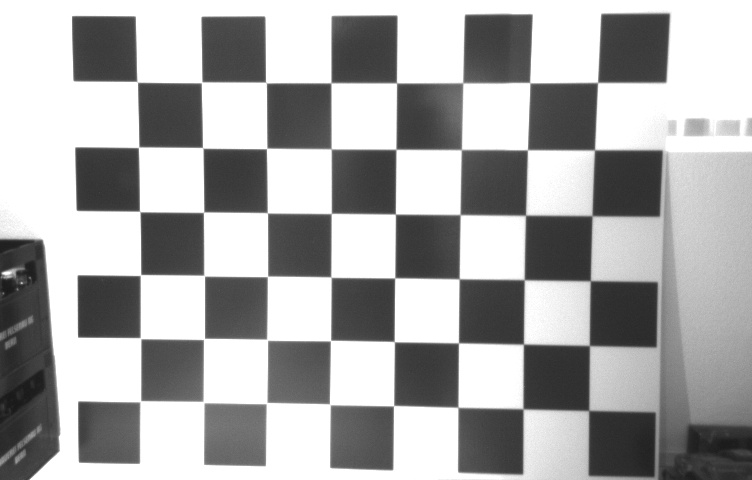
\includegraphics[width=0.4\textwidth]{img/calib0_left.jpg}}
	\subfloat[right image used for calibration]{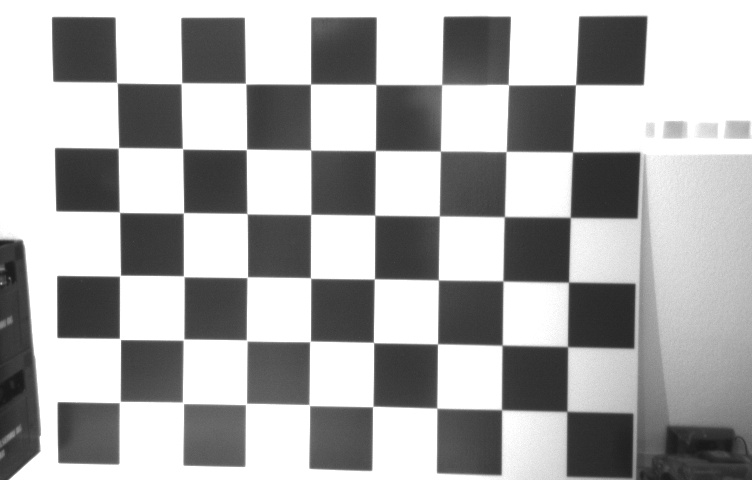
\includegraphics[width=0.4\textwidth]{img/calib0_right.jpg}}\\
	\subfloat[left image after rectification]{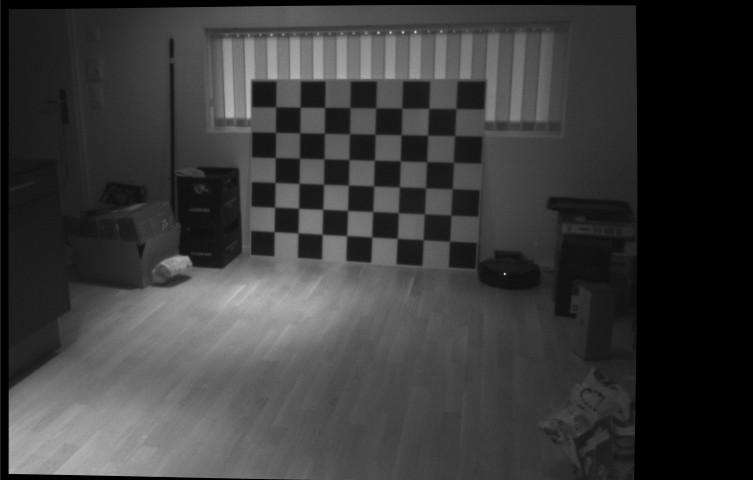
\includegraphics[width=0.4\textwidth]{img/calib0_left_rect.jpg}}
	\subfloat[right image after rectification]{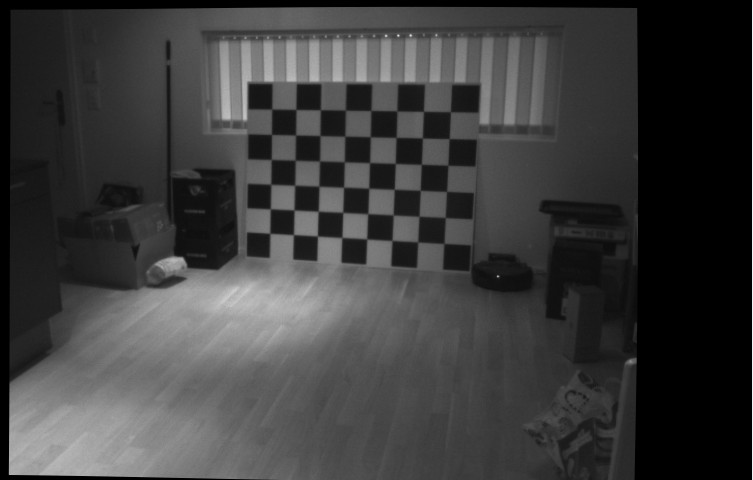
\includegraphics[width=0.4\textwidth]{img/calib0_right_rect.jpg}}
	\caption{Top: Two images used to calibrate the camera, Bottom: New images after rectify}\label{fig:calibration_real}
\end{figure}

Figure \ref{fig:calibration_real} shows a ``real'' example of a calibrated stereo camera. In comparison to example \ref{fig:stereo_calib} this calibration also corrects distortion and equalizes fx and fy for both cameras. Only rectified images as shown in figure \ref{fig:calibration_real} are used for SLAM in the following chapters. The images are rectified right after capturing from camera.\\

Another parameter stereo calibration can calculate is the baseline between both cameras. The baseline is the distance of the centers of the left and the right camera. For that we have to specify the length of one checkerboard field. With known size we can calculate the baseline. However, the calibration process will output focal length in pixels times baseline in meters as shown in equation \ref{eq:bf}. As we will see in equation \ref{eq:depth} this is the value needed for calculating the depth from disparity.

\begin{equation}\label{eq:bf}
	b_f=\frac{b*f}{p_s}
\end{equation}

\begin{align*}
	b_f &:	\text{Output of calibration process}\\
	b &:		\text{basline in m}\\
	f &:		\text{focal lenght in m}\\
	p_s &:	\text{Pixel size in m}\\
\end{align*}

\section{Checkerboard Size}

For camera calibration it is important to use a big checkerboard. The bigger the board the better the calibration result gets. The reason is hidden in equation \ref{eq:cm}. When we try to find the projection matrix we will always have a small error. This error comes from restrictions regarding resolution and misplacement while detecting corners. However, if the checkerboard is far away the error will be divided through the distance because we are not interested in scale while doing camera calibration. This means the farer away the checkerboard is the smaller will be the influence of our error.\\
For calibrating the camera we printed a checkerboard onto an advertisement board as offered by \cite{mydisplay}.\\
To see how well the calibration process performs we have to analyze the reprojection error that can be received by stereoCalibExtended of OpenCV. The error should be below 0.5 pixels, the smaller the better.\\
For calibrating the Econ Tara, a checkerboard of size $1500x1000mm$ was used. The Checkerboard fields have a size of $166x166mm$ which leads to $8x6$ inner corners detectable by the calibration script described in the next section.

\section{Econ Tara calibration}
For calibrating the Econ Tara camera we can use the econ\_calibration\_images.py script. We find this script in the project repo under test \cite{pa2}.
\begin{lstlisting}[language=bash]
python3 econ_calibration_images.py <calib folder> --size <field size>
\end{lstlisting}

<field size> is the height and width of one checkerboard field. The images in the folder <calib folder> are gray scale and have the form <name><counter>\_left and <name><counter>\_right. We can use the script extract\_channels.py to create the images:
\begin{lstlisting}[language=bash]
python3 extract_channels.py <camera> <hidraw> <calib folder>
\end{lstlisting}
This script expects the path to the Econ Tara camera, the path to the hidraw device (to set auto-exposure) and the output folder. Pressing "w" in the image preview will save a new image. Pressing "q" will quit the program.

\chapter{ORB SLAM}\label{chap:implementation}

In this chapter we discuss more deeply how ORB SLAM works and how we port it to the iMX8 processor.

\section{How it works}
ORB SLAM tries to find corners with FAST corner detection \cite{fast}. This gives us points which should lay on the intersection between two edges. We call this points keypoints. At this points we calculate the ORB descriptors \cite{orb} which describe the keypoints in a unique way. Based on this keypoints ORB SLAM will estimate the pose and position of the camera in various steps shown in figure \ref{fig:orb_slam2}.

\begin{figure}[H]
  \begin{center}
		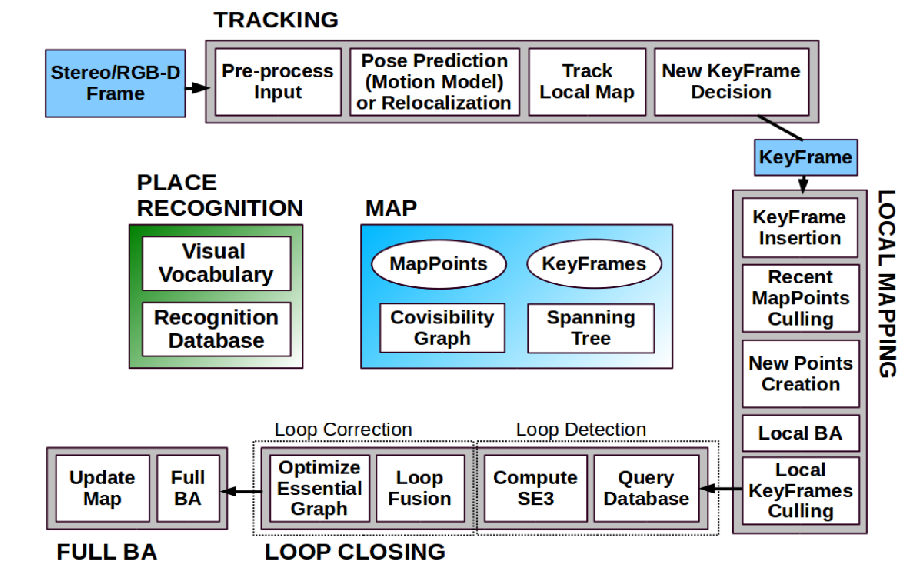
\includegraphics[width=0.9\textwidth]{img/orb_slam2.png}
  \end{center}
	\caption{ORB SLAM 2 \cite{orbslam2}}\label{fig:orb_slam2}
\end{figure}

ORB SLAM uses multiple threads to improve the performance of the algorithm, this threads and it's tasks are described in the following sections.

\begin{figure}[H]
  \begin{center}
		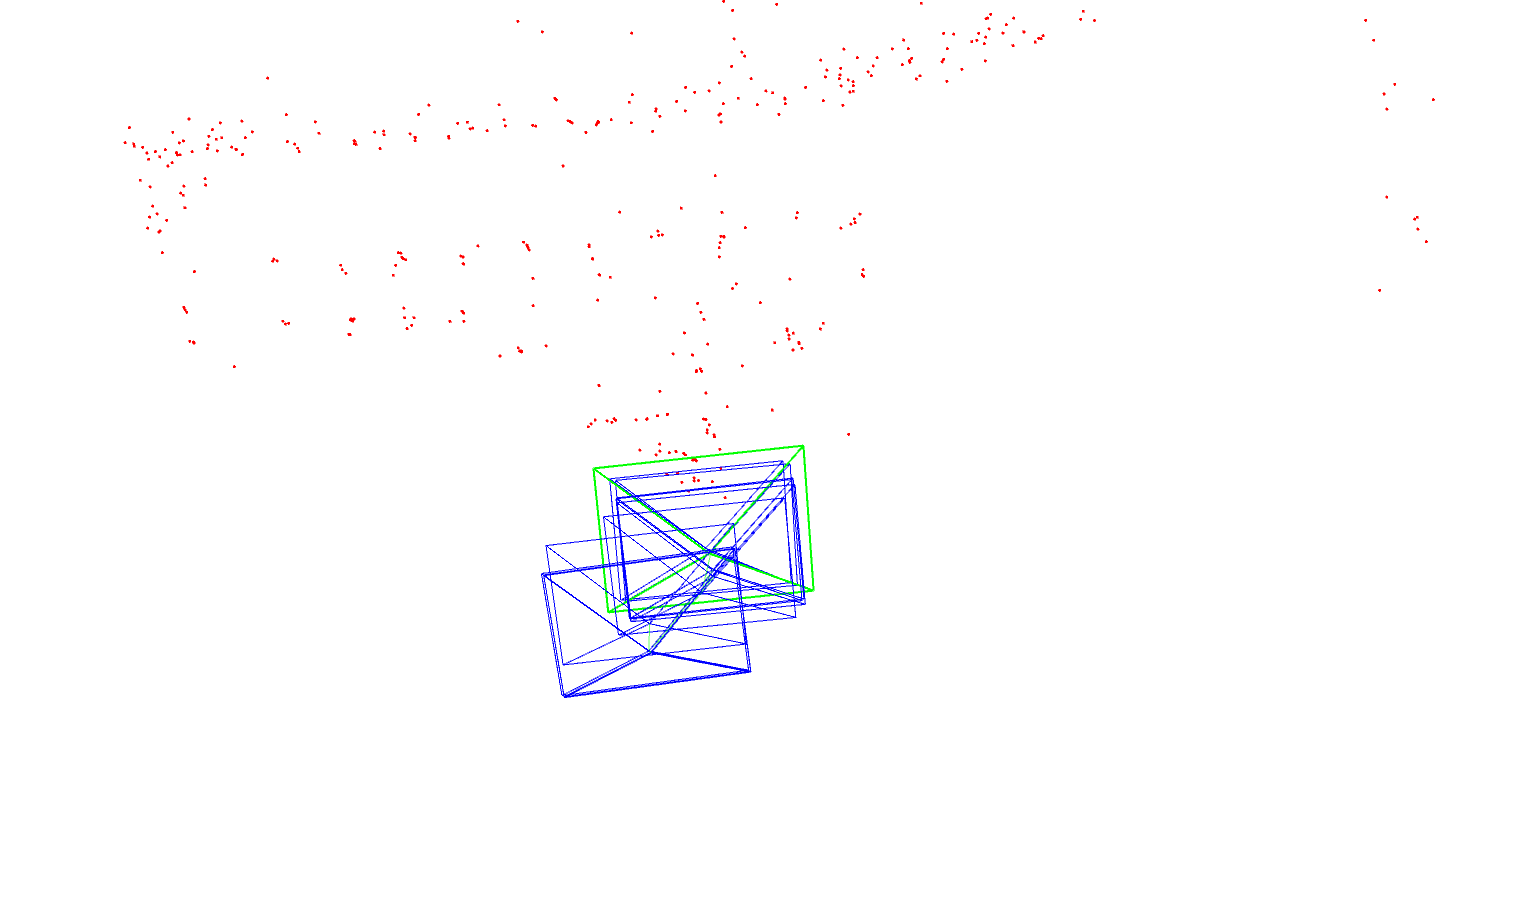
\includegraphics[width=0.9\textwidth]{img/pose_map.png}
  \end{center}
	\caption{ORB SLAM 2 keyframes (blue), keypoints (red) current camera view (green)}\label{fig:pose_map}
\end{figure}

In the following section we will use the terms keypoints, keyframes, pose and position. In figure \ref{fig:pose_map} we see what this terms mean. The pose and position is where the image was taken and in which direction the camera was looking. Pose and position is equivalent to the extrinsic camera matrix.

\subsection{Initialization}

Before starting with tracking the system needs an initialization step. In this step it generates the first point cloud with camera at origin. For stereo SLAM this step is simple:
\begin{enumerate}
	\item Calculate ORB keypoints on the left and right image
	\item Match the ORB descriptors of both images
	\item Calculate the disparity (difference) in pixel between the left and right image of each point
	\item Calculate depth with equation \ref{eq:depth}
	\item Calculate x and y position with equation \ref{eq:orb_pos}
\end{enumerate}	

\begin{equation}\label{eq:depth}
\begin{aligned}
	d&=\frac{f*b}{p_s*\Delta}\\
	\Delta&=x_{left}-x_{right}
\end{aligned}
\end{equation}
\begin{align*}
	d &:					\text{depth}\\
	b &:					\text{baseline in m}\\
	f &:					\text{Focal length in m}\\
	p_s	&:				\text{Pixel size in m}\\
	\Delta &:			\text{Disparity}\\
	x_{left} &:		\text{X Position of keypoint on left image}\\
	x_{right} &: 	\text{X Position of keypoint on right image}
\end{align*}

\begin{equation}\label{eq:orb_pos}
\begin{aligned}
	X&=\frac{d*x}{f_x}\\
	Y&=\frac{d*y}{f_y}
\end{aligned}
\end{equation}
\begin{align*}
	X &:				\text{X position with camera as origin}\\
	Y &: 				\text{Y position with camera as origin}\\
	d &: 				\text{Depth=Z position with camera as origin}\\
	x,y &:			\text{x,y position in pixels in the image}\\
	f_x,f_y &:	\text{Focal length}
\end{align*}

This gives us an initial point cloud with camera as origin. We use this point cloud to estimate further poses as described in the following section. We will also have a look at the differences between stereo and monocular initialization in section \ref{sec:monster}.

\subsection{Tracking}

Tracking is the most important task where the algorithm estimates the pose and position of the current camera view. It performs the following steps:
\begin{enumerate}
	\item Find ORB keypoints on both images
\end{enumerate}

With known motion model from previous tracking:
\begin{enumerate}
	\setcounter{enumi}{1}
	\item Search for matching ORB descriptors based on motion model
	\item If the movement goes to the right we take the left image for the search if the movement goes to the left we take the right image
	\item Backproject points from 3D cloud with projection matrix found with motion model
	\item Optimize pose and position with Levenberg Marquardt \cite{levenbergmarquardt} to minimize the backprojection error
	\item Calculate the motion model by using the pose and position of the previous and current frame
\end{enumerate}

With unknown motion model:
\begin{enumerate}
	\setcounter{enumi}{1}
	\item Search best matching keyframe with DBoW2 \cite{dbow}
	\item Match ORB descriptors with best fitting keyframe
	\item Triangulate the current pose as described in section \ref{sec:triangulation}
	\item Calculate the motion model by using the pose and position of the previous and current frame
\end{enumerate}

At the end we check if the current frame is a potential keyframe. We do this by checking how many frames were captured since the last keyframe, if a lot of outliers were detected and if more than 35\% of points are new with regards to the reference keyframe. If it fulfills everything the new frame is a possible keyframe.\\

\subsection{Local Mapping}
Local mapping tries to map the newly found keypoints into the world map. It only does local mapping for possible keyframes found in the previous step.
\begin{enumerate}
	\item Transform new keypoints to the global coordinate system based on the camera pose
	\item Do bundle adjustment \cite{bundleadjustment}. It is likely that points we already know do not 100\% match the position where we see the points. Bundle adjustment fuses the position of points found more than once.
	\item Check if more than 10\% of the points in the current frame compared to the points in all keyframes are new. If not we drop the keyframe.
\end{enumerate}

\subsection{Loop Closing}
Loop closing tries to detect loops and will then do a bundle adjustment to increase the precision of the point cloud.
\begin{enumerate}
	\item Match latest keyframe with all keyframes stored in the database with DBoW2 \cite{dbow}
	\item Check if the match closes a loop
	\item Optimize corresponding points by doing bundle adjustment over all keyframe poses and point positions
\end{enumerate}

Loop Closing increases the precision of the point cloud because it can remove drift. However, it only takes effect if a loop is detected as shown in figure \ref{fig:loop_closing}.

\begin{figure}[H]
  \begin{center}
		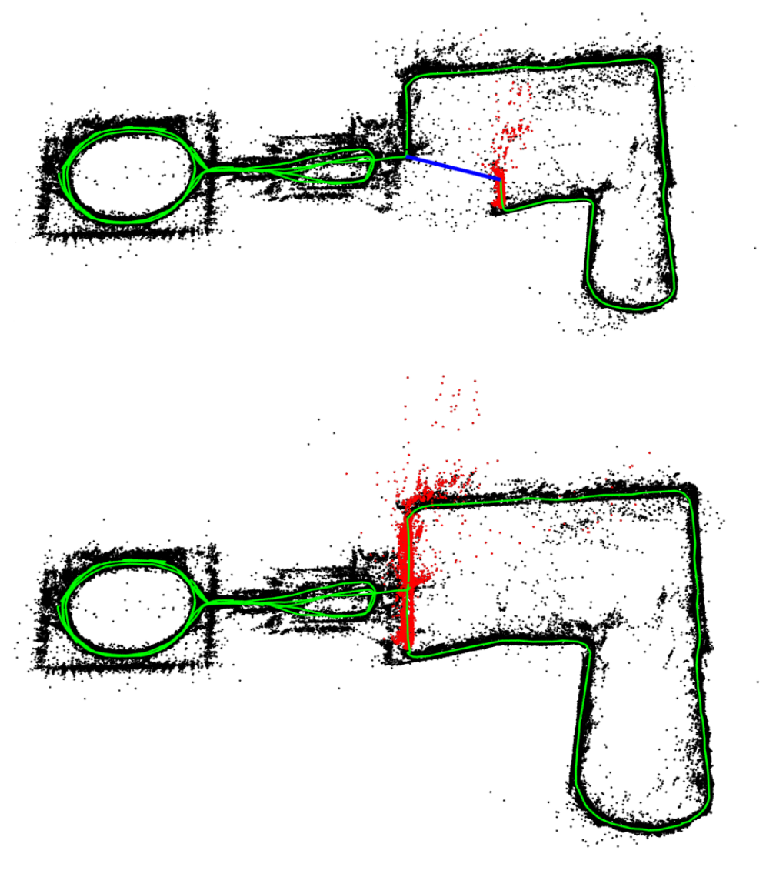
\includegraphics[width=0.9\textwidth]{img/loop_closing.jpg}
  \end{center}
	\caption{A map before (top) and after (bottom) loop closing. The blue line shows the error before bundle adjustment.}\label{fig:loop_closing}
\end{figure}

\subsection{Triangulation}\label{sec:triangulation}

Triangulation is the step where we find a projection matrix based on a 3D/2D point mapping. We have to know at least 6 points for doing triangulation with the linear model. By doing triangulation we want to find the projection matrix $p_{ij}$ in \ref{eq:projection}.

\begin{equation}\label{eq:projection}
	\begin{pmatrix}p_{11} & p_{12} & p_{13} & p_{14}\\
		p_{21} & p_{22} & p_{23} & p_{24}\\
		p_{31} & p_{32} & p_{33} & p_{34}\\
	\end{pmatrix}*
	\begin{pmatrix}
		X \\
		Y \\
		Z \\
		1
	\end{pmatrix}=
	\begin{pmatrix}
		u \\
		v \\
		s
  \end{pmatrix}
\end{equation}
Where:
\begin{align*}
	p_{ij}		&: \text{Unknown camera projection values of projection matrix P}\\
	X,Y,Z			&: \text{3D Point}\\
	u,v,s			&: \text{2D Point}\\
\end{align*}

We can rewrite equation \ref{eq:projection} as shown in equation \ref{eq:projection_flat}. We don't know u and v directly. We only have the pixel position which is $x=u/s, y=v/s, 1$. There is no way to estimate s. We know that s equals to the third row of equation \ref{eq:projection_flat}. If we multiply x and y by the third row, the equation will still hold (equation \ref{eq:projection_flat_s}). As a side effect we can remove the third row because the left and right side are equal which always holds. We finally have two equation per image point. Another trick we use is to set $p_{34}$ to 1. This makes the Z position of the camera the norm for the other unknowns. Because of this change the trivial solution where every unknown is zero disappears. We can solve the final equation \ref{eq:projection_flat_red} for all unknowns $p_{ij}$ with linear least square.

% Make sure we can have the whole column matrix (normally a line break will follow after 10 columns)
\setcounter{MaxMatrixCols}{15}
\begin{equation}\label{eq:projection_flat}
	\begin{pmatrix}
		X & Y & Z & 1 & 0 & 0 & 0 & 0 & 0 & 0 & 0 & 0\\
		0 & 0 & 0 & 0 & X & Y & Z & 1 & 0 & 0 & 0 & 0\\
		0 & 0 & 0 & 0 & 0 & 0 & 0 & 0 & X & Y & Z & 1\\
	\end{pmatrix}
	\begin{pmatrix}p_{00}\\
		p_{11}\\
		p_{12}\\
		p_{13}\\
		p_{14}\\
		p_{21}\\
		p_{22}\\
		p_{22}\\
		p_{23}\\
		p_{31}\\
		p_{32}\\
		p_{33}\\
		p_{34} \\
	\end{pmatrix}=
	\begin{pmatrix}u\\
		v\\
		s\\
	\end{pmatrix}
\end{equation}

\begin{equation}\label{eq:projection_flat_s}
	\begin{pmatrix}u\\
		v\\
		s\\
	\end{pmatrix}=\begin{pmatrix}
		x*(X*p_{31}+Y*p_{32}+Z*p_{33}+p_{34})\\
		y*(X*p_{31}+Y*p_{32}+Z*p_{33}+p_{34})\\
		1*(X*p_{31}+Y*p_{32}+Z*p_{33}+p_{34})
	\end{pmatrix}
\end{equation}


\begin{equation}\label{eq:projection_flat_red}
	\begin{pmatrix}
		X & Y & Z & 1 & 0 & 0 & 0 & 0 & -xX & -xY & -xZ\\
		0 & 0 & 0 & 0 & X & Y & Z & 1 & -yX & -yY & -yZ
	\end{pmatrix}
	\begin{pmatrix}
		p'_{00}\\
		p'_{11}\\
		p'_{12}\\
		p'_{13}\\
		p'_{14}\\
		p'_{21}\\
		p'_{22}\\
		p'_{23}\\
		p'_{24}\\
		p'_{31}\\
		p'_{32}\\
		p'_{33}
	\end{pmatrix}=
	\begin{pmatrix}x\\
		y\\
	\end{pmatrix}
\end{equation}
Where:
\begin{align*}
	p_{ij}		&: \text{unknown camera projection values}\\
	p'_{ij}		&: \text{same as c but normalized to $p_{34}$}\\
	X,Y,Z			&: \text{3D Point}\\
	u,v,s			&: \text{2D Point with scale factor s}\\
	x,y				&: \text{2D Point normalize to s=1}\\
\end{align*}

We miss one last step. We set $p_{34}$ to 1 to get rid of the trivial solution where all $p_{ij}$ are zero. We now have to find the right value for $p_{34}$. If we calculate the intrinsic times the extrinsic matrix we end up in equation \ref{eq:ext_int}. We focus on the third row. We know that the norm of a column of a rotation matrix must be one. The reason for this is that a rotation matrix will never change the length of a vector. Therefore, $h=\sqrt{r_{31}^2+r_{32}^2+r_{33}^2}$ must be one \cite{Wu}. Because we normalized tz to one, this assumption does not hold for our solution. The camera distance $t_z$ will therefore be $1*1/h$. To correct the projection matrix we can multiply the matrix with $1/h$ (equation \ref{eq:ext_int_scaled}).

\begin{equation}\label{eq:ext_int}
	P=
	\begin{pmatrix}
		f_xr_{11}+p_xr_{31} & f_xr_{12}+p_xr_{32} & f_xr_{13}+p_xr_{33} & f_xt_x+p_xt_z\\
		f_yr_{21}+p_yr_{31} & f_yr_{22}+p_yr_{32} & f_yr_{23}+p_yr_{33} & f_yt_y+p_yt_z\\
		r_{31} & r_{32} & r_{33} & t_z
	\end{pmatrix}
\end{equation}

\begin{equation}\label{eq:ext_int_scaled}
	P=1/h
	\begin{pmatrix}
		p'_{11} & p'_{12} & p'_{13} & p'_{14}\\
		p'_{21} & p'_{22} & p'_{23} & p'_{24}\\
		p'_{31} & p'_{32} & p'_{33} & 1\\
	\end{pmatrix}
\end{equation}

Where:
\begin{align*}
	P					&: \text{projection matrix}\\
	p_{ij}'		&: \text{projection matrix found with $t_z=1$}\\
	f_x,f_y		&: \text{focal length}\\
	c_x,c_y		&: \text{principal point}\\
	r_{ij}		&: \text{Parameters of rotation matrix}\\
	t_{x,y,z}	&: \text{location of the camera}\\
	h					&: \text{scaling inverse $tz=1/\sqrt{r_{31}^{'2}+r_{32}^{'2}+r_{33}^{'2}}$}
\end{align*}


Now that we know all unknowns we can calculate the extrinsic matrix that describes the pose. We need to multiply the inverse intrinsic matrix times the projection matrix as shown in equation \ref{eq:extrinsic}. If we prefere angles instead of the rotation matrix we can extract them as shown in equation \ref{eq:angles}. Equation \ref{eq:angles_proof} shows the rotation matrix derived from angles. To get back angles we use the fact that $arctan(sin(x)/cos(x))=x$.
\begin{equation}\label{eq:angles_proof}
\begin{aligned}
	&R=\begin{pmatrix}
		&c(\theta_y)c(\theta_z) & -c(\theta_y)s(\theta_z) & s(\theta_y)\\
		&c(\theta_x)s(\theta_z)s(\theta_y)c(\theta_z) & c(\theta_x)c(\theta_z)-s(\theta_x)s(\theta_y)s(\theta_z) & -s(\theta_x)c(\theta_y)\\
		&s(\theta_x)s(\theta_z)-c(\theta_y)c(\theta_z) & c(\theta_x)s(\theta_y)s(\theta_z)+s(\theta_x)c(\theta_z) &	c(\theta_x)c(\theta_y)\\
	\end{pmatrix}
\end{aligned}
\end{equation}
Where:
\begin{align*}
	\theta_n	&: \text{Rotation in n direction}\\
	s				  &: \text{sin}\\
	c				  &: \text{cos}\\
\end{align*}

From that we get:
\begin{equation}\label{eq:angles}
\begin{aligned}
	\theta_y &= arcsin(sin(\theta_y)) = arcsin(r_{02})\\
	\theta_x &= arctan(\frac{-sin(\theta_x)cos(\theta_y)}{cos(\theta_x)cos(\theta_y)}) = arctan(\frac{r_{12}}{r_{22}})\\
	\theta_z &= arctan(\frac{-cos(\theta_y)sin(\theta_z)}{cos(\theta_y)cos(\theta_z)}) = arctan(\frac{r_{01}}{r_{00}}) 
\end{aligned}
\end{equation}
Where:
\begin{align*}
	\theta_n	&: \text{Rotation in n direction}\\
	r_{nn}	  &: \text{Rotation matrix term see equation \ref{eq:cm}}\\
\end{align*}

Because we normally have more than 6 points available for triangulation we use RANSAC \cite{ransac} to find a good solution and to eliminate outliers.

\section{Comparison Mono to Stereo}\label{sec:monster}

In this work we only talk about stereo SLAM. But what are the differences to a monocular SLAM system?\\
A monocular camera can't see depth. This means that from one single image we can't estimate the keypoints in the 3D world. Therefore, we need an initialization process that will try to estimate the depth over several images. There are different strategies for solving the initialization problem. ORB SLAM calculates two models in parallel one when most points are laying on a plane and one model when most points are randomly distributed. In one model we search the essential matrix (fundamental matrix with 5 DoF) in the other we search the homography matrix \cite{orbslam}. If the initialization succeeds one of this matrices will converge to a small reprojection error while the other wont. The camera pose and position is calculated by decomposing the converged matrix.\\
Other approaches use an extended Kalman filter (EKF) and try to optimize the camera pose over the first n frames \cite{svo}. The EKF starts with points at random depth values and converges after several frames to the ``real'' depth values. For a monocular camera it is not possible to find all 6 DoF because the fundamental and homography matrix only have 5 DoF. They therefore set the 6 parameter to 1 which means we don't get a real ``scale'' value. All measurements with monocular cameras will therefore have an unknown scale.

\section{Port to iMX8}\label{sec:orbport}

The iMX8 BSP is built with Yocto. NXP and Toradex provide a BSP layer which contains a kernel and all necessary proprietary libraries for OpenGL. How we build the BSP and the SDK is out of scope of this project. We find more details about the BSP under the following references:
\begin{itemize}
	\item Yocto project \cite{yocto}
	\item Toradex BSP \cite{toradex_bsp}
\end{itemize}

From the Yocto build we can also get an SDK which contains an ARM64 toolchain that can be used to compile additional programs and libraries. This toolchain was used to build ORB SLAM 2 for iMX8. For the following section we assume that the toolchain is installed under /opt/fsl-imx-x11/4.9.51-mx8-beta.

\subsection{Pangolin}
Pangolin \cite{pangolin} is required by ORB SLAM for showing the sparse map and the camera pose. A simple git checkout of the pangolin sources is enough to receive the sources. Before building the project with CMake the following patch should be applied:
\begin{lstlisting}
diff --git a/CMakeLists.txt b/CMakeLists.txt
index 32a2d78..683ef38 100644
--- a/CMakeLists.txt
+++ b/CMakeLists.txt
@@ -15,6 +15,9 @@ SET(CPACK_DEBIAN_PACKAGE_MAINTAINER "Steven Lovegrove")
 SET(CPACK_PACKAGE_VERSION_MAJOR ${PANGOLIN_VERSION_MAJOR})
 SET(CPACK_PACKAGE_VERSION_MINOR ${PANGOLIN_VERSION_MINOR})
 SET(CPACK_PACKAGE_VERSION_PATCH "0")
+SET(CMAKE_INCLUDE_SYSTEM_FLAG_CXX "-I")
+SET(CMAKE_INCLUDE_SYSTEM_FLAG_C "-I")
+
 include(CPack)
 
 option( BUILD_EXAMPLES "Build Examples" ON )
\end{lstlisting}

After that the following commands will compile and install Pangolin:
\begin{lstlisting}[language=bash]
. /opt/fsl-imx-x11/4.9.51-mx8-beta/environment-setup-aarch64-poky-linux
mkdir build
cd build
cmake -DCMAKE_INSTALL_PREFIX=<INSTALL_DIR> ..
make -j
make install
\end{lstlisting}

This will build the Pangolin library for ARM64. INSTALL\_DIR should point to a directory which is used as local ``root filesystem''. This root filesystem should be copied via scp to the iMX8.

\subsection{OpenCV}\label{sec:opencv}
We modified ORB SLAM 2 for this project by adding different ORB implementations and by adding Densification. To make this version work we need the modified OpenCV version from \cite{opencv_se}. The branch se-3.4.3 contains some modification which allows to reuse the image pyramid generated by ORB. Also the CMake flags are changed to allow compilation on iMX8. Additionally we need to compile OpenCV Contribute \cite{opencv_contrib} version tag 3.4.3. To build OpenCV plus OpenCV Contribute the following commands are required:
\begin{lstlisting}[language=bash]
. /opt/fsl-imx-x11/4.9.51-mx8-beta/environment-setup-aarch64-poky-linux
. /opt/fsl-imx-x11/4.9.51-mx8-beta/sysroots/x86_64-pokysdk-linux/\
environment-setup.d/cmake.sh

mkdir build
cd build

export PKG_CONFIG_LIBDIR="/opt/fsl-imx-x11/4.9.51-mx8-beta/\
sysroots/aarch64-poky-linux/usr/lib/pkgconfig/"
cmake -DWITH_ITT=NO -DWITH_LIBV4L=YES -DWITH_TBB=NO\
 -DOPENCV_EXTRA_MODULES_PATH=<path to OpenCV contrib>\
 -DCMAKE_BUILD_TYPE=Release ..
\end{lstlisting}

We need to copy all libraries found in the lib directory to the iMX8.

\subsection{ORB SLAM 2}\label{sec:orbslam_build}
The sources of this project are based on ORB SLAM 2 \cite{orbslam2_impl}. Instead of using the sources of the original implementation, the modified sources \cite{orbslam2_se} under branch work\_se should be used. They contain some fixes for newer compiler versions as well as additional sources for the Econ Tara camera. After fetching the sources with git the following commands will build the binary:\\
\begin{lstlisting}[language=bash]
. /opt/fsl-imx-x11/4.9.51-mx8-beta/environment-setup-aarch64-poky-linux
mkdir build
cd build
cmake -DPangolin_DIR=<INSTALL_DIR/usr/lib/cmake/Pangolin>\
 -DCMAKE_INSTALL_PREFIX=<INSTALL_DIR>\
 -DOpenCV_DIR:PATH=<OPENCV_BUILD_DIR> ..
make -j
make install
\end{lstlisting}

This will build ORB SLAM for ARM64. INSTALL\_DIR is the same directory as it was for Pangolin. After that we can copy the whole INSTALL\_DIR to the iMX8 root directory and start econ\_stereo to start the SLAM system. The OPENCV\_BUILD\_DIR should point to the build directory of OpenCV in section \ref{sec:opencv}.

\subsection{ORB SLAM 2 usage}

For the Econ Tara a special stereo\_econ application is available. This application can be called as follows:
\begin{lstlisting}[language=bash]
./stereo_econ path_to_vocabulary path_to_settings path_to_video
\end{lstlisting}

The first argument path\_to\_vocabulary points to the ORB dictionary for DBoW2, path\_to\_settings should point to the Econ.yaml and path\_to\_video points to the Econ stereo camera device.\\
In comparison to the orignal ORB SLAM 2 implementation some additional parameters are added:\\
\begin{tabular}{l l}
stereosgbm.cn & CN parameter fo sgbm \\
stereosgbm.preFilterCap & Pre filter capacity for sgbm \\
stereosgbm.windowSize & Window size for sgbm \\
stereosgbm.blockSize & Block size for sgbm \\
stereosgbm.minDisparity & Minimum disparity for sgbm \\
stereosgbm.speckleRange &  Speckle Range for sgbm \\
stereosgbm.disp12MaxDiff & Max diff for sgbm \\
stereosgbm.uniquenessRatio & Uniqueness ratio for sgbm \\
stereosgbm.speckleWindowSize & Speckle window size for sgbm \\
stereosgbm.numberOfDisparities & Total number of disparities for sgbm \\
cpu.system & CPU assigned to system thread \\
cpu.stereoleft & CPU assigned to ORB thread for left image \\
cpu.stereoright & CPU assigned to ORB thread for right image \\
cpu.loopclosing & CPU assigned to loop closing thread \\
cpu.localmapping & CPU assigned to local mapping thread \\
cpu.densify & CPU assigned to densify thread \\
cpu.viewer & CPU assigned to viewer \\
Densify.enabled & 0 if densify is disabled 1 if enabled \\
ORBextractor.orbextractor & Orb extractor:\\
													& 0->Original, 1->OpenCV, 2->OpenCV OCL \\
Densify.topmargin & top margin for depth image \\
Densify.bottommargin & bottom margin for depth image \\
Densify.leftmargin & left margin for depth image \\
Densify.rightmargin & right margin for depth image \\
\end{tabular}\\

The SGBM features are hard to tune the values in Econ.yaml were taken from the stereo\_match.cpp example of OpenCV \cite{opencv_se}. The ORBextractor.orbextractor can be used to switch between different ORB implementations in section \ref{sec:results}. Densify.*margin is used to add margins to depth images. This is necessary because points close to the boarder have higher uncertainty.

\chapter{Densification}

\begin{figure}[H]
  \begin{center}
		\includegraphics[width=0.9\textwidth]{img/dense_cloud.png}
  \end{center}
	\caption{A dense cloud generated with SGBM and ORB SLAM}\label{fig:dense_cloud}
\end{figure}

ORB SLAM only delivers a sparse map. This sparse map can't be used for creating maps or to reconstruct 3D objects. The focus of ORB SLAM is to find a stable pose and position of the camera. In this section we discuss how we can improve ORB SLAM by densifing the point cloud as shown in figure \ref{fig:dense_cloud}. We also will show a first implementation that is part of the modified ORB SLAM sources (see section \ref{sec:orbslam_build}).\\
In the first section we see how the stereo images can be used to create a depth map. The next section describes how to use the depth map to generate a point cloud. The two last sections discuss two possibilities on how a depth map of several poses could be fused together. However, as we will see the current approach doesn't work as expected because the point cloud size increases too fast. Therefore, we don't have CPU time to fuse the point clouds effectively.

\section{Depth Map}

A depth map is an image that contains depth values instead of color intensities. They are generated from stereo cameras or from ToF cameras. We will only talk about how depth images are made from stereo cameras. Image \ref{fig:depth}c shows a depth image made from two stereo images.

\begin{figure}[H]
	\centering
	\subfloat[left image]{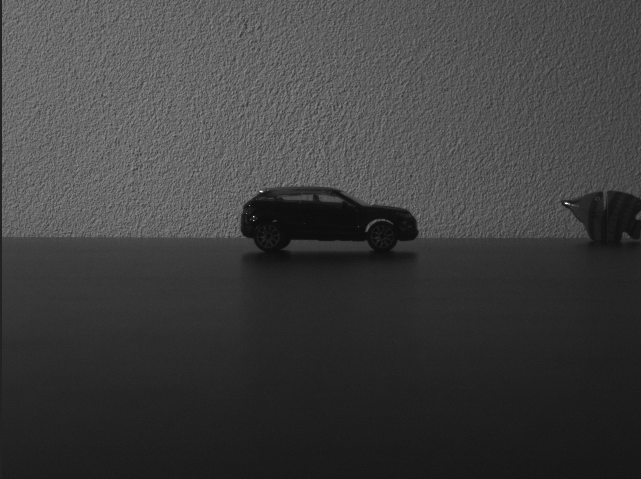
\includegraphics[height=100px]{img/disparity_left.png}}
	\subfloat[right image]{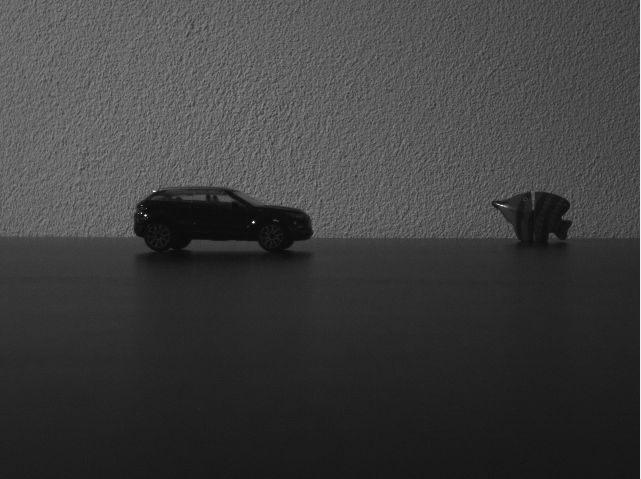
\includegraphics[height=100px]{img/disparity_right.png}}
	\subfloat[depth image]{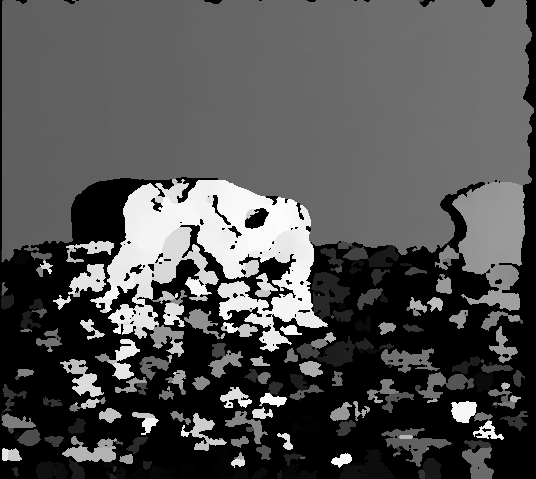
\includegraphics[height=100px]{img/disparity.png}}
	\caption{Depth image from stereo}\label{fig:depth}
\end{figure}

The algorithm for crating depth images matches the intensities of the left and right images. Because we vertically aligned the camera, the algorithm starts matching the right image at pixel position of the left image and searches from there to the right as shown in figure \ref{fig:disparity}. The position with the least intensity difference between left and right is where we calculate the distance. We call the distance between the left and right image disparity. An object far away has less disparity than a near object. A point at infinity will have a disparity of zero. As we see in figure \ref{fig:depth} the depth image is noisy in areas where we have low or no texture. To reduce the influence of noise, the algorithm not only matches the intensity at one pixel, it uses a block of several pixels instead (e.g. 9x9).
\begin{figure}[H]
  \begin{center}
		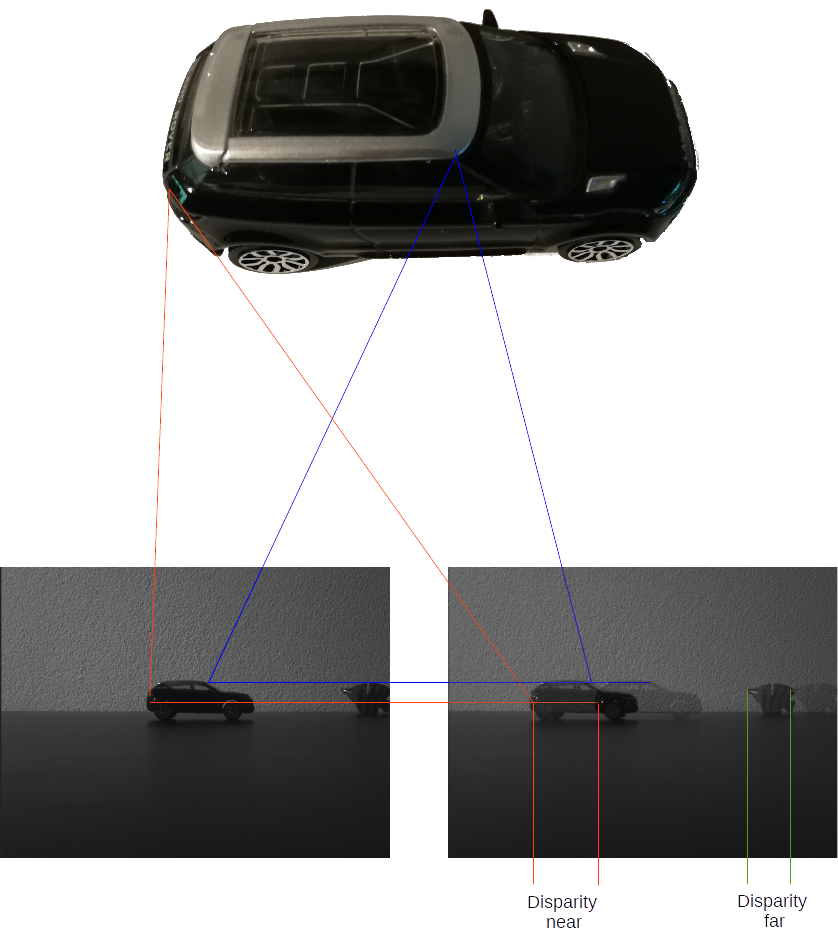
\includegraphics[width=0.9\textwidth]{img/disparity_concept.png}
  \end{center}
	\caption{Disparity with epipolar (horizontal) line, left: left image, right: right image with transparent left image}\label{fig:disparity}
\end{figure}

As described we calculate the disparity by doing block matching. However, this algorithm is still prone to noise. Therefore, we use a modified version of this algorithm called Semi Global Block Matching (SGBM) \cite{sgbm}. Compared to normal block matching this algorithm penalties big disparity differences between neighbouring pixels. We also calculate the disparity for the left and right image to get values for pixels only visible in one image. Further we generate a confidence map if pixels have different disparities when we do left and right matching. We use this confidence map to filter vague disparities and replace them with values of their neighbourhood.

\section{Point Cloud from Depth}

From the depth map generated by the previous section we calculate a dense point cloud based on the current pose. We transform the depth information into the three dimensional space. An example of such a point cloud is shown in figure \ref{fig:pointcloud}. The point cloud is generated from the depth image by multiplying each pixel with the current camera pose.

\begin{equation}\label{eq:point_cloud_depth}
	\begin{pmatrix}
			X' \\
			Y' \\
			Z'
	\end{pmatrix}=
	\begin{pmatrix}
		r_{00} & r_{01} & r_{02} & t_x \\
		r_{10} & r_{11} & r_{12} & t_y \\
		r_{20} & r_{21} & r_{22} & t_z \\
	\end{pmatrix}*
	\begin{pmatrix}
		X\\
		Y\\
		d\\
		1\\
	\end{pmatrix}
\end{equation}
\begin{align*}
	X',Y',Z' &:		\text{World position of the pixel}\\
	r_{ij} &:			\text{Rotation of extrinsic camera matrix}\\
	t_{x,y,z} &:	\text{Translation of extrinsic camera matrix}\\
	X,Y &:				\text{X,Y with current view as origin, see \ref{eq:orb_pos}}\\
	d &:					\text{Depth or Z value with current view as orign}
\end{align*}

\begin{figure}[H]
  \begin{center}
		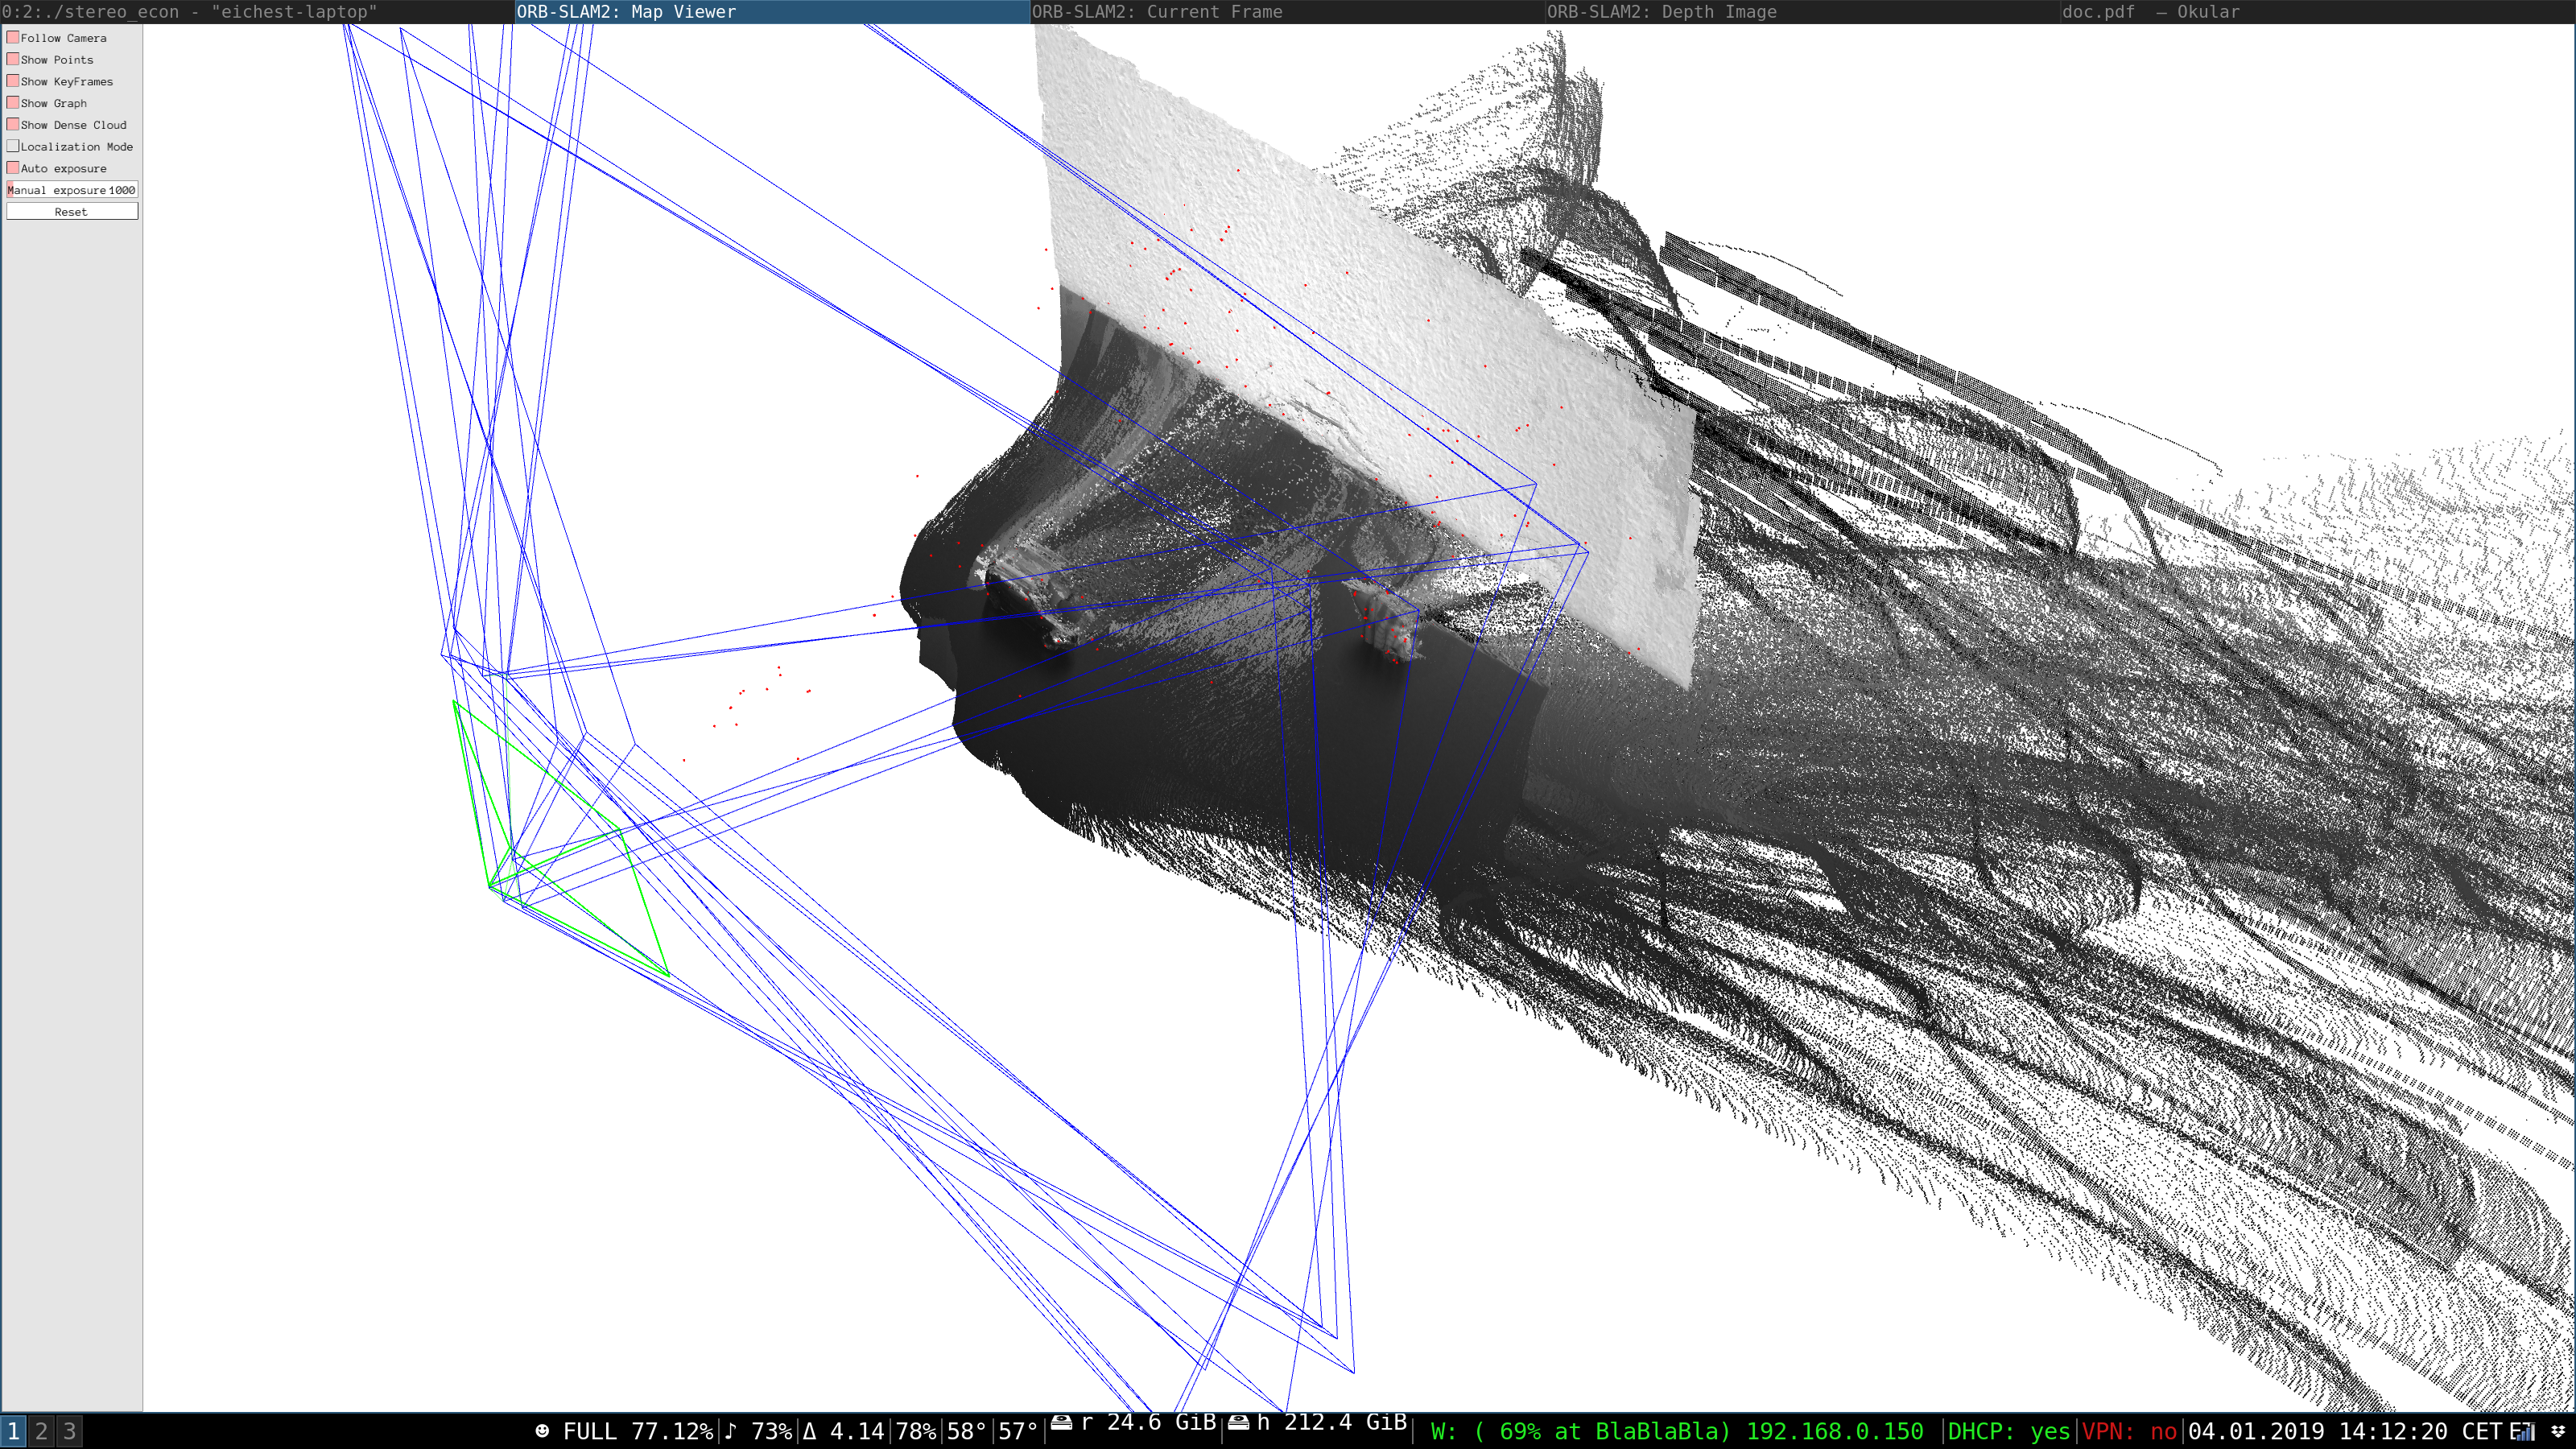
\includegraphics[width=0.9\textwidth]{img/pointcloud.png}
  \end{center}
	\caption{Dense point cloud generated from different keyframes}\label{fig:pointcloud}
\end{figure}

To reduce the CPU load, we add new dense points to the cloud only for keyframes. What we see in figure \ref{fig:pointcloud} is that because of the uncertainty of the depth map we have tons of outliers. Further we don’t fuse points at the same location therefore we generate a lot of points that have the same position within a statistical uncertainty.

\section{Point Cloud fusion}

There are different papers that describe the problem of point cloud fusion. If we have two views that partially show the same region we have to merge the overlapping part. This section describes two methods to fuse point clouds. REMODE is a probabilistic approach while volumetric 3D mapping is a more direct approach.

\subsection{REMODE}

REMODE \cite{remode} uses a probabilistic approach to fuse data from different views. Only points with high enough probability are drawn on the 3D map. This generates a semi-dense point cloud which has a high probability of being true. However, it requires a lot of frames seeing the same scene for getting high accuracy, this is exactly what we try to avoid because we already have problems to perform well with our current approach. Therefore, this algorithm isn’t suitable for us.

\subsection{Volumetric 3D Mapping}

Volumetric 3D Mapping \cite{volumetric} is designed to run on a CPU. It assigns a box to each 3D pixel and puts this box into an octree. If we want to add a new pixel, the algorithm checks whether it fits in an existing box. Unfortunately, a proof of concept implementation showed that even with this approach the CPU load explodes when using one point for each image pixel.

\chapter{Discussion}

In this chapter we discuss the status of the work. We analyse the current results and see if we can improve ORB SLAM to perform at 20fps.

\section{Results}\label{sec:results}

The current implementation is heavily based on the original ORB SLAM 2 implementation as described in section \ref{sec:orbport}. Because we used normal ORB SLAM the results from the original paper are still valid. However, what we are interested in is the realtime frame rate and therefore the time used per frame for tracking. The ORB SLAM 2 implementation for standard datasets calculates this time and prints the mean and median time after each run. For comparison we used the KITTI04 dataset with 271 images. The resolution of each image is 1226x370 where the ECON Tara has a resolution of 752x480. The KITTI dataset is a standard benchmark for SLAM therefore it was taken. In comparison to Euroc another dataset it has smaller sequences and finishes therefore faster.\\\

We compare the ORB SLAM ORB implementation with the ORB implementation from OpenCV. To be fair we reduce the feature count when using OpenCV from 1000 to 800 because OpenCV ORB finds more features than the ORB SLAM implementation. The bigger the point cloud gets the slower the algorithm becomes, therefore tracking more features wouldn't be a fair comparison.\\

\begin{table}
	\begin{tabular}{  | l | l | l | l | l | l | }
		\hline
		\textbf{CPU} & \textbf{Impl.} & \textbf{feat.} & \textbf{feat. det.} & \textbf{med. tt} & \textbf{mean tt} \\ \hline
		iMX8 & ORB & 1000 &  548 & 0.18307 & 0.185202 \\ \hline
		iMX8 & ORB, Lin. sched. & 1000 & 548 & 0.390867 & 0.387753 \\ \hline
		iMX8 & OpenCV & 1000 & 757 & 0.190571 & 0.210072 \\ \hline
		iMX8 & OpenCV & 800 & 610 & \textbf{0.155441} & \textbf{0.167176} \\ \hline
		iMX8 & OpenCV, Lin. sched. & 800 & 610 & 0.358689 & 0.362126 \\ \hline
		iMX8 & OpenCV OpenCL & 800 & 610 & 0.50622 & 0.771859 \\ \hline
		i5-7Y54 & ORB & 1000 & 546 & 0.18884 & 0.184628 \\ \hline
		i5-7Y54 & OpenCV & 1000 & 756 & 0.154901 & 0.152786 \\ \hline
		i5-7Y54 & OpenCV & 800 & 610 & 0.135715 & 0.132304 \\ \hline
	\end{tabular}
	\caption{Comparison of ORB SLAM tracking time in KITTI04 using ORB or OpenCV implementation}
  \label{tab:result}
\end{table}

As we see from table \ref{tab:result} we achieve best timings on the iMX8 when using the OpenCV ORB SLAM implementation. We could extend this version that it behaves the same as the ORB SLAM implementation and would still performs better. However, we are still at a low frame rate of around 6 frames per seconds. When we compare the results of the iMX8 to a i5-7Y54 Intel processor, we see similar results with around 7fps. Unfortunately, none of these result is near to 20fps. We consider 20fps as realtime because our eye would recognize that as fluent. 6-7fps work well for slow movements but the system can’t handle fast movements because of the bad performance. The biggest disappointment is that the OpenCL implementation of ORB in OpenCV is worse than the CPU implementation. We therefore can’t increase the performance by using the GPU instead of the CPU.\\
What we also see in table \ref{tab:result} is a speciality of the iMX8. The Linux scheduler isn't aware that this processor has two different processor types. Therefore, it can't move a task which requires a fast CPU to a Cortex A72 processor. We therefore added the possibility to the ORB SLAM configuration file to bind a task to a specific processor. This allows us to use the two Cortex A72 for tracking and other high performance tasks. We see that when relying on Linux scheduler the tracking time nearly doubles. This isn't a problem on the Intel processor, because all processors are of the same type.  

\section{Optimizations}

The current frame rate on the iMX8 as well as on a laptop CPU is too low. This makes it hard to get a robust tracking and mapping.

\subsection{Different ORB Implementation}
To increase the performance we can use a different ORB implementation. By using the OpenCV ORB implementation we see that higher frame rates are possible. However, this improves the performance only by around 20\%. To get to 20fps we would have to improve the performance by factor 4.

\subsection{Using OpenCL}
OpenCV ORB supports finding FAST corners and calculating ORB descriptor with OpenCL. However, a first test showed that using OpenCL is even slower than using the CPU. So this approach doesn't look promising for now.

\subsection{Reduce Resolution}
Using lower resolution images would improve the performance of the algorithm. However, this is not something we want to do because it also decreases the stability. With a resolution of 752x480 we already limit the resolution to a realistic level for embedded devices.

\subsection{Using a different SLAM algorithm}
Because we don't see too many options to improve ORB SLAM a different SLAM algorithm could be used. We will discuss that in chapter \ref{chap:direct}.

\section{Problems}

In this section we try to describe some problems of ORB SLAM.

\subsection{Complexity}
ORB SLAM has grown to a complex algorithm. It's therefore hard to trace the algorithm in detail and to find bottlenecks. The use of multi threading increases the complexity even more.

\subsection{Tracking}
For our use case we don't need a full SLAM algorithm and tracking would be sufficient. Because we do densification we won't necessarily benefit of bundle adjustment, because this would invalidate the dense cloud. When doing tracking based on a motion model we don't benefit from ORB descriptors.

\subsection{Old dependencies}
ORB SLAM depends on old libraries this generates a lot of warnings while compiling. To use it in a serious project, we would have to eliminate this warnings.

\subsection{Slow compilation}
Modifying ORB SLAM is a pain. Recompiling ORB SLAM takes a lot of time because it uses libeigen which heavily uses templates. Maybe this could be improved by fixing include directives.

\subsection{Workflow}
For doing proof of concepts C++ is a heavy and unflexible language. A mix between scriptable (e.g. Python or Matlab) and compilable (e.g. C++) language could improve the workflow.

\chapter{Direct Approach}\label{chap:direct}
Because a lot of new papers describe sparse direct approaches as faster than indirect methods we analyze one of them. This could be the basis for further work specially when using it in combination with data from an IMU.

\section{SVO}

SVO \cite{svo} stands for sparse visual odometry. It is a sparse direct approach to the SLAM problem. The first monocular implementation was released as open source. The improved SVO2 source code is not publicly available. However, the paper describes the algorithm in detail so it should be possible to do a similar implementation. We can describe the main parts of the algorithm as follows.

Initialization (Stereo):
\begin{enumerate}
	\item Search corner points with FAST
	\item Split the image into areas of fixed size (e.g. 32x32)
	\item Take the FAST corner with maximum response in each area if there is any
	\item (optional) If there is no FAST corner take the point with highest gradient on an edge (see \ref{fig:svo})
	\item With a stereo camera we can do a block matching for each of this ~100 points to find the depth
	\item Add current frame as keyframe
\end{enumerate}

Tracking:
\begin{enumerate}
	\item For each point we try to minimize the photometric error (intensity difference)
	\item We use a motion model received from previous tracking as initial pose and position to optimize it with Levenberg-Marquardt
		\subitem (optional) The motion model can be improved with an IMU
	\item (optional) For each point we calculate the backprojection into the image
	\item (optional) For each point we search the minimal intensity difference within a small window around the backprojection
	\item (optional) We calculate the difference of the position from backprojection and intensity search
	\item (optional) We adjust the 3D points with bundle adjustment to minimize the mismatch between position of the backprojection and position found by intensity search.
\end{enumerate}

\begin{figure}[H]
  \begin{center}
		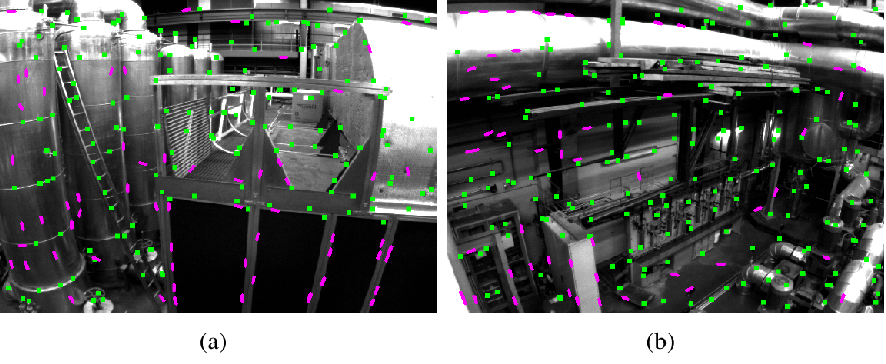
\includegraphics[width=1.0\textwidth]{img/svo.png}
  \end{center}
	\caption{Example of sparse points used by SVO in Euroc dataset \cite{svo}. The green points are fast corners the magenta points are edgelets used in areas with no corners}\label{fig:svo}
\end{figure}

This algorithm can't do loop closing as ORB SLAM does. However, it would be possible to add such improvement if necessary (e.g. by using ORB descriptors only on keyframes). Due to it's simplicity they report 13.27ms to process one 640x480 frame in EUROC Machine Hall 1 on a Nvidia Jetson TX1. The CPU of this processor is comparable to the one on the iMX8. This would end up in a frame rate up to 75fps which is above 60fps, the maximum of the Econ camera.

\section{Densification}

The SVO paper describes the possibility to do densification based on sparse points. Another problem however is that dense clouds consume a lot of memory, which is not something you have granted on embedded systems. Because SVO uses corners as key points an approach could be to generate a mesh between all keypoints. To get a better feeling of the environment, keyframes can serve as textures to render a 3D map. To increase the resolution we need to get closer to the object, with a closer view we will detect more keypoints in the same area which makes the cloud denser. With this approach we don't need a point for each pixel. This reduces the CPU and memory consumption and gives room to do filter operations (like plane detection) on the 3D cloud.

\section{Outlook}
SVO SLAM is especially interesting because of its simplicity and because it is possible to remove a lot of optional features. By removing this optional features the tracking results become worse. If we combine tracking with data from IMU, we can hopefully compensate the loss of precision. Together with a stereo camera we also don’t need the complicated initialization process described in the SVO paper because we can directly calculate the depth of each point with the first frame.

\chapter{Conclusion}
The current results for ORB SLAM show it is not convenient for embedded devices. It is hard to optimize the algorithm because of its complexity. Even with multi-threading and multiprocessing in place we can’t speed up the algorithm to over 10 frames per second. Therefore, we propose to analyze a direct sparse approach in further work for doing SLAM instead of using an indirect sparse approach. The disadvantage of being computationally more expensive in point matching is compensated by the advantage of not having the need to extract expensive features. We showed that we can reduce SVO to a simple implementation when not using all optional features. We therefore propose to use SVO in further work for doing SLAM and to generate a mesh from keypoints found by SVO. This mesh can be used as map for navigating a robot around obstacles.

\listoffigures
 
\begin{thebibliography}{1}

	\bibitem{orb}
	E. Rublee, V. Rabaud, K. Konolige, and G. Bradski\\
	\textit{ORB: an efficient alternative to SIFT or SURF}\\
	IEEE International Conference on Computer Vision (ICCV), Barcelona, Spain, November 2011, pp. 2564–2571.

  \bibitem{orbslam}
  Raul Mur-Artal, J. M. M. Montiel, Juan D. Tardos\\
  \textit{ORB-SLAM: a Versatile and Accurate Monocular SLAM System}\\
  arXiv:1502.00956v2

  \bibitem{orbslam2}
  Raul Mur-Artal, J. M. M. Montiel, Juan D. Tardos\\
  \textit{ORB-SLAM2: an Open-Source SLAM System for Monocular, Stereo and RGB-D Cameras}\\
	arXiv:1610.06475v2 

	\bibitem{dtam}
	Richard A. Newcombe, Steven J. Lovegrove and Andrew J. Davis\\
	\textit{DTAM: Dense Tracking and Mapping in Real-Time}\\
	doi:10.1109/ICCV.2011.6126513

	\bibitem{svo}
	Christian Forster et al\\
	\textit{SVO: Semi-Direct Visual Odometry for Monocular and Multi-Camera Systems}\\
	doi:10.1109/TRO.2016.2623335

	\bibitem{fast}
	E. Rosten, R. Porter, and T. Drummond \\
	\textit{Faster and better: A machine learning approach to corner detection}\\
	doi:10.1109/TPAMI.2008.275

	\bibitem{mvg}
	Richard Hartley\\
	\textit{Multiple View Geometry in Computer Vision}\\
	ISBN-10: 0-511-18618-5, p240-249

	\bibitem{levenbergmarquardt}
	Wikipedia\\
	\textit{Levenberger-Marquardt algorithm}\\
	https://en.wikipedia.org/wiki/Levenberg\%E2\%80\%93Marquardt\_algorithm

	\bibitem{zed}
	Stereo Labs\\
	\textit{ZED Stereo Camera}\\
	https://www.stereolabs.com/zed/

	\bibitem{tara}
	Econ\\
	\textit{Tara Stereo Camera}\\
	https://www.e-consystems.com/3D-USB-Stereokamera-de.asp

	\bibitem{realsense}
	Intel\\
	\textit{Intel RealSense}\\
	https://realsense.intel.com/depth-camera/\#D415\_D435


	\bibitem{opencv_calib}
	OpenCV\\
	\textit{Camera Calibration}\\
	https://docs.opencv.org/3.4.3/dc/dbb/tutorial\_py\_calibration.html

	\bibitem{mydisplay}
	mydisplay.ch\\
	\textit{Advertisement board manufacturer}\\
	https://www.mydisplays.ch/

	\bibitem{yocto}
	Yocto Project\\
	\textit{Yocto Project Mega Manual}\\
	https://www.yoctoproject.org/docs/latest/mega-manual/mega-manual.html

	\bibitem{toradex_bsp}
	Toradex AG\\
	\textit{Build Apalis iMX8 OpenEmbedded Project Bring-up Image}\\
	https://developer.toradex.com/software/linux/linux-software/build-apalis-imx8-yoctoopenembedded-bring-up-image

	\bibitem{dbow}
	D. Gálvez-López and J. D. Tardós\\
	\textit{Bags of binary words for fast place recognition in image sequences}\\
	IEEE Trans. Robot., vol. 28, no. 5, pp. 1188–1197, 2012.

	\bibitem{sgbm}
	Heiko Hirschmüller\\
	\textit{ Stereo Processing by Semi-Global Matching and Mutual Information}\\
	IEEE TRANSACTIONS ON PATTERN ANALYSIS AND MACHINE INTELLIGENCE
	 
	\bibitem{rvc}
	Peter Corke\\
	\textit{Robotics, Vision and Control}\\
	Springer, ISBN 978-3-319-54413-7, chapter 11+12, page 319+

	\bibitem{ransac}
	wikipedia\\
	\textit{RANSAC}\\
	https://de.wikipedia.org/wiki/RANSAC-Algorithmus

	\bibitem{bundleadjustment}
	B. Triggs, P. F. McLauchlan, R. I. Hartley, and A. W. Fitzgibbon\\
	\textit{Bundle adjustment a modern synthesis}\\
 	in Vision algorithms: theory and practice, 2000, pp. 298–372. 

	\bibitem{Wu}
	Ying Wu,\\
	\textit{Image Formation and Camera Calibration}\\
	http://users.eecs.northwestern.edu/~yingwu/teaching/EECS432/Notes/camera.pdf 

	\bibitem{remode}
	Pizzoli, Matia and Forster, Christian and Scaramuzza, Davide\\
	\textit{REMODE: Probabilistic, Monocular Dense Reconstruction in Real Time}\\
	IEEE International Conference on Robotics and Automation (ICRA), 2014

	\bibitem{volumetric}
	Frank Steinbrücker, Jürgen Sturm, Daniel Cremers\\
	\textit{Volumetric 3D mapping in real-time on a CPU}\\
	doi:10.1109/ICRA.2014.6907127

	\bibitem{pangolin}
	Steven Love Grove\\
	\textit{Pangolin Project}\\
	https://github.com/stevenlovegrove/Pangolin.git

  \bibitem{orbslam2_impl}
  Raul Mur-Artal, J. M. M. Montiel, Juan D. Tardos\\
  \textit{ORB-SLAM2 Implemenation}\\
	https://github.com/raulmur/ORB\_SLAM2

  \bibitem{orbslam2_se}
  Raul Mur-Artal, J. M. M. Montiel, Juan D. Tardos\\
  \textit{ORB-SLAM2 Implemenation modified version}\\
	https://github.com/eichenberger/ORB\_SLAM2.git

	\bibitem{opencv_se}
	OpenCV\\
	\textit{OpenCV computer vision framework (modified version)}\\
	https://github.com/eichenberger/opencv

	\bibitem{opencv_contrib}
	OpenCV\\
	\textit{OpenCV computer vision framework extensions}\\
	https://github.com/opencv/opencv\_contrib
	
	\bibitem{pa2}
	Stefan Eichenberger\\
	\textit{Project 2: ORB Slam Point Cloud generation on Apalis iMX8}\\
	https://github.com/eichenberger/pa2

\end{thebibliography}


\end{document}
